\section{El Espacio Afín Euclídeo.}\label{Rel:Tema2}

\begin{ejercicio}
    Sean $\cc{A}$ un espacio afín euclídeo y S un subespacio afín suyo. Dado un punto $p \in \cc{A}$ demuestra que existe $q_0 \in S$ tal que
    \begin{equation*}
        d(p, q_0) = d(p, S) := \inf\{d(p, q) : q \in S\}.
    \end{equation*}

    Demostramos en primer lugar que existe $q_0 \in S$ tal que $\vec{pq_0}\in \vec{S}^\perp$.
    Notemos el subespacio $S$ como $S=q+\vec{S}$.
    
    Como se tiene que $\vec{\cc{A}}=\vec{S}\oplus \vec{S}^\perp$, entonces $\exists_1 u\in \vec{S}, v\in \vec{S}^\perp$ tal que:
    \begin{equation*}
        \vec{pq} = u+v
    \end{equation*}

    Sea $q_0=q-u\in S$. Entonces:
    \begin{equation*}
        v = \vec{pq}-u = q-p-u = q_0-p = \vec{pq_0} \in \vec{S}^\perp
    \end{equation*}

    Veamos ahora que $d(p,q_0)\leq d(p,q)~ \forall q\in S$:
    \begin{multline*}
        d^2(p,q) = \langle\vec{pq}, \vec{pq}\rangle
        = \langle\vec{pq_0} + \vec{q_0q}, \vec{pq}+ \vec{q_0q}\rangle
        = \|\vec{pq_0}\|^2 + \|\vec{q_0q}\|^2 + 2\cancel{\langle\vec{pq_0}, \vec{q_0q}\rangle} =\\= \|\vec{pq_0}\|^2 + \|\vec{q_0q}\|^2 \geq \|\vec{pq_0}\|^2 = d^2(p,q_0) \qquad \forall q\in S
    \end{multline*}

    Por tanto, $d(p,q_0)$ es un minorante del conjunto. Como además $q_0\in S$, pertenece al conjunto, por lo que es el ínfimo. Por tanto, se tiene.
\end{ejercicio}

\begin{ejercicio}[Hiperplano afín de puntos equidistantes] Dados tres puntos $p, q, r \in~\bb{R}^n$, demostrar que se cumple la igualdad
    \begin{equation*}
        d(p,q)^2 - d(q,r)^2 = 2\langle\vec{rm_{pq}}, \vec{qp}\rangle,
    \end{equation*}
    donde $m_{pq}$ es el punto medio entre $p$ y $q$. Utilizar esta igualdad para probar lo siguiente: si $p \neq q$, entonces el conjunto de los puntos de $\bb{R}^n$ que se encuentran a la misma distancia de $p$ y de $q$ coincide con el hiperplano $m_{pq} + \cc{L}(\{\vec{p q}\})^\perp$.

    Demostrado en la Proposición \ref{prop:caract_mediatriz}, ya que el hiperplano descrito es la mediatriz de $p$ y $q$.
\end{ejercicio}

\begin{ejercicio}
    Dados los siguientes pares de rectas de $\bb{R}^2$, estudia su posición relativa. Si se cortan, determina el ángulo que forman; en otro caso, calcula la distancia entre ellas.
    \begin{enumerate}
        \item $R=\{(x,y)\in \bb{R}^2 \mid x=y\}$, $S=\{(x,y)\in \bb{R}^2\mid 2x-y=0\}$.

        Tenemos que $R=(0,0)+\cc{L}\{(1,1)\}$, $S=(0,0)+\cc{L}(1,2)$. 

        Por tanto, son secantes. El origen $(0,0)\in S\cap R$ está en la intersección. Veamos el ángulo entre las rectas:
        \begin{equation*}
            \frac{\langle (1,1), (1,2)\rangle}{\|(1,1)\|~\|(1,2)\|} = \frac{1+2}{\sqrt{2}\cdot \sqrt{5}} = \frac{3}{\sqrt{10}}
            \hspace{2cm}
            \frac{\langle (1,1), -(1,2)\rangle}{\|(1,1)\|~\|-(1,2)\|} = -\frac{3}{\sqrt{10}}
        \end{equation*}

        Por tanto, tenemos que el ángulo es:
        \begin{equation*}
            \alpha = \measuredangle (S,R) = \arccos \left(\frac{3}{\sqrt{10}}\right) \approx 0.32~ \text{rad}
        \end{equation*}
        
        \item $R=\{(x,y)\in \bb{R}^2 \mid x-y=1\}$, $S=\{(2\lambda,1+2\lambda) \mid \lambda\in \bb{R}\}$.

        Tenemos que $S=\{(x,y)\in \bb{R}^2\mid y=1+x\}=\{(x,y)\in \bb{R}^2\mid x-y=-1\}$. Por tanto, como las ecuaciones cartesianas de $S\cap R$ forman un SI, tenemos que $S\cap R=\emptyset$. Calculamos la distancia entre ambas rectas.

        Tenemos que $R=\{(\mu, \mu-1)\mid \mu\in \bb{R}\}=(0,-1)+\cc{L}\{(1,1)\}$. Además, $S=(0,1)+\cc{L}\{(1,1)\}$. Por tanto, un vector arbitrario que una ambas rectas es $v=\vec{(\mu,\mu-1)(2\lm, 1+2\lm)}=(2\lm-\mu, 2\lm -\mu + 2)$. Como $v\in \vec{R}^\perp$, entonces:
        \begin{equation*}
            \langle (2\lm-\mu, 2\lm -\mu + 2), (1,1)\rangle = 0
            \Longleftrightarrow 4\lm -2\mu +2 = 0
        \end{equation*}

        Por ejemplo, para $\lm = 0$, $\mu=1$ se tiene que $v\in \vec{R}^\perp = \vec{S}^\perp$, tenemos que:
        \begin{equation*}
            d(R,S) = \|v\| = \|(-1, 1)\| = \sqrt{2}
        \end{equation*}
    \end{enumerate}
\end{ejercicio}

\begin{ejercicio}
    En el espacio vectorial $\cc{P}_2(\bb{R})$, consideramos el producto escalar definido como $\langle p(x), q(x)\rangle = \int_0^1 p(x)q(x)~dx$.
    Dotamos $\cc{P}_2(\bb{R})$ de la estructura afín canónica (que lo convierte en un espacio afín euclídeo) y consideramos las siguientes rectas afines:
    \begin{equation*}
        S = \{p(x) \in \cc{P}_2(\bb{R}) \mid p(0) = 5, p''(8) = 4\}
        \qquad \text{y} \qquad
        T = \langle\{5x^2 - 2x, 2x^2 - x + 1\}\rangle.
    \end{equation*} 
    Comprueba si $S$ y $T$ se cortan en un punto, y en dicho caso calcula el ángulo que forman.\\

    Buscamos obtener las ecuaciones cartesianas de $S$. Tenemos que $p\in \cc{P}_2(\bb{R})$ arbitrario es $p(x)=a_0+a_1x+a_2x^2$, con $a_0,a_1,a_2\in \bb{R}$. Además, $p'(x)=a_1+2a_2x$ y $p''(x)=2a_2$. Por tanto, las condiciones dadas son $a_0=5,~ a_2=2$. Por tanto, las ecuaciones paramétricas de $S$ en el sistema de referencia $\cc{R}=\{0,\cc{B}_u=\{1,x,x^2\}\}$ son:
    \begin{equation*}
        S = \{(a_0,a_1,a_2)_{\cc{R}}\in \cc{P}_2(\bb{R})\mid a_0=5,~a_2=2\}
    \end{equation*}

    Respecto a $T$, tenemos que el vector director es:
    $$\vec{(5x^2-2x)(2x^2-x+1)} = (2x^2-x+1) - (5x^2-2x) = -3x^2+x+1$$

    Por tanto, $T=5x^2-2x + \cc{L}\{-3x^2+x+1\}$. Para calcular las ecuaciones cartesianas en $\cc{R}$, el rango de la siguiente matriz ha de ser 1, para que
    los vectores sean linealmente dependientes:
    \begin{equation*}
        rg\left(
            \begin{array}{cc}
                1 & 0-a_0 \\
                1 & -2-a_1\\
                -3 & 5-a_2
            \end{array}
        \right) = 1
    \end{equation*}

    Para ello, ha de ser:
    \begin{equation*}
        \left|
            \begin{array}{cc}
                1 & 0-a_0 \\
                1 & -2-a_1\\
            \end{array}
        \right| = 0 = -2-a_1 + a_0 = 0
        \qquad \qquad
        \left|
            \begin{array}{cc}
                1 & 0-a_0 \\
                -3 & 5-a_2
            \end{array}
        \right| = 0 = 5-a_2-3a_0 = 0
    \end{equation*}

    Por tanto, las ecuaciones cartesianas en $\cc{R}$ son:
    \begin{equation*}
        T = \{(a_0,a_1,a_2)_{\cc{R}}\in \cc{P}_2(\bb{R})\mid a_0-a_1=2,~3a_0+a_2=5\}
    \end{equation*}

    Por tanto, las ecuaciones cartesianas de $S\cap T$ en $\cc{R}$ son:
    \begin{equation*}
        S\cap T = \{(a_0,a_1,a_2)_{\cc{R}}\in \cc{P}_2(\bb{R})\mid a_0 = 5,~a_1=3,~a_2=2,~3a_0+a_2=5\}
    \end{equation*}

    Por tanto, $S\cap T = \emptyset$, por lo que no se cortan.
\end{ejercicio}

\begin{ejercicio}
    En el espacio vectorial $\cc{M}_{2\times 2}(\bb{R})$, consideramos el producto escalar definido como $\langle M, N\rangle = tr(M^tN)$. Dotamos $\cc{M}_{2\times 2}(\bb{R})$ de la estructura afín canónica (que lo convierte en un espacio afín euclídeo). Calcula el ángulo que forman los siguientes hiperplanos afines:
    \begin{equation*}
        S = \{M \in \cc{M}_{2\times 2}(\bb{R}) \mid tr(M) = 2\}
        \quad \text{y}\quad 
        T = \left\{\left(\begin{array}{cc}
            a & b \\ c & d
        \end{array}\right) \in \cc{M}_{2\times 2}(\bb{R}) \mid a = 1 \right\}
    \end{equation*}


    Tenemos que $S$ viene dado por:
    \begin{equation*}
        S = \left\{\left(\begin{array}{cc}
            a & b \\ c & d
        \end{array}\right) \in \cc{M}_{2\times 2}(\bb{R}) \mid a + d = 2 \right\}
    \end{equation*}

    Tenemos que los vectores normales a $S$ y $T$, que son:
    \begin{equation*}
        n_S=\left(\begin{array}{cc}
            1 & 0 \\ 0 & 1
        \end{array}\right)
        \hspace{1cm}
        n_T=\left(\begin{array}{cc}
            1 & 0 \\ 0 & 0
        \end{array}\right)
    \end{equation*}

    Entonces $\measuredangle(S,T) = \measuredangle (n_S, n_T)$, por lo que:
    \begin{equation*}
        \measuredangle(S,T) = \arccos \left(\frac{tr(n_S^tn_T)}{tr(n_S^tn_S) \cdot tr(n_T^tn_T)}\right)
        = \arccos \left(\frac{1}{2 \cdot 1}\right) = \frac{\pi}{3}
    \end{equation*}
\end{ejercicio}


\begin{ejercicio}
    En $\bb{R}^2$ consideramos dos triángulos $T_1 = \{a_1, a_2, a_3\}$ y $T_2=~\{b_1, b_2, b_3\}$. Demuestra que:
    \begin{enumerate}
        \item Existen seis aplicaciones afines de $\bb{R}^2$ en $\bb{R}^2$ que llevan $T_1$ en $T_2$.

        Son las distintas formas de reordenar el conjunto de 3 elementos; es decir, las permutaciones, que son $3!=6$.
        Estas son:
        \begin{equation*}
            \begin{array}{l}
                f_1(a_1) = b_1,\quad f_1(a_2) = b_2,\quad f_1(a_3) = b_3 \\
                f_2(a_1) = b_1,\quad f_2(a_2) = b_3,\quad f_2(a_3) = b_2 \\
                f_3(a_1) = b_2,\quad f_3(a_2) = b_1,\quad f_3(a_3) = b_3 \\
                f_4(a_1) = b_2,\quad f_4(a_2) = b_3,\quad f_4(a_3) = b_1 \\
                f_5(a_1) = b_3,\quad f_5(a_2) = b_1,\quad f_5(a_3) = b_2 \\
                f_6(a_1) = b_3,\quad f_6(a_2) = b_2,\quad f_6(a_3) = b_1
            \end{array}
        \end{equation*}

        \item Una de las aplicaciones afines anteriores $f : \bb{R}^2 \to \bb{R}^2$ es isometría si y sólo si
        \begin{equation*}
            d(a_i, a_j ) = d(f(a_i), f(a_j )), \qquad \forall i, j \in \{1, 2, 3\},
        \end{equation*}
        donde $d(\cdot, \cdot)$ es la función distancia de $\bb{R}^2$.

        \begin{description}
            \item[$\Longrightarrow)$] Por ser isometría, se tiene de forma directa.
            \item[$\Longleftarrow)$] Supongamos que se cumple la igualdad. Entonces, tenemos que:
            \begin{equation*}
                d(a_i, a_j) = d(f(a_i), f(a_j)) \qquad \forall i,j\in \{1,2,3\}
            \end{equation*}

            Por tanto, $f$ es una aplicación afín que preserva la distancia entre los vértices del triángulo.
            Veamos que $f$ preserva la distancia entre dos puntos cuales quiera
            $p,q\in \bb{R}^2$. Para ello, usamos que $\cc{R}=\left\{a_1, \left\{\vec{a_1a_2}, \vec{a_1a_3}\right\}\right\}$ es un sistema de referencia de $\vec{\bb{R}^2}$, por lo que:
            \begin{align*}
                p &= a_1 + \alpha_1\vec{a_1a_2} + \alpha_2\vec{a_1a_3} \qquad \alpha_1,\alpha_2\in \bb{R}
                \\
                q &= a_1 + \beta_1\vec{a_1a_2} + \beta_2\vec{a_1a_3} \qquad \beta_1,\beta_2\in \bb{R}
            \end{align*}

            Entonces:
            \begin{align*}
                d(p,q) &= \left\|\vec{pq}\right\| = \left\|q-p\right\| = \left\|(\beta_1-\alpha_1)\vec{a_1a_2} + (\beta_2-\alpha_2)\vec{a_1a_3}\right\|
                \leq\\&\leq  |\beta_1-\alpha_1|\cdot \left\|\vec{a_1a_2}\right\| + |\beta_2-\alpha_2|\cdot \left\|\vec{a_1a_3}\right\|
            \end{align*}
            \begin{align*}
                d(f(p),f(q)) &= \left\|\vec{f(p)f(q)}\right\| = \left\|\vec{f}\left(\vec{pq}\right)\right\|
                =\\&= \left\|(\beta_1-\alpha_1)\vec{f}\left(\vec{a_1a_2}\right) + (\beta_2-\alpha_2)\vec{f}\left(\vec{a_1a_3}\right)\right\|
                \leq\\&\leq  |\beta_1-\alpha_1|\cdot \left\|\vec{f}\left(\vec{a_1a_2}\right)\right\| + |\beta_2-\alpha_2|\cdot \left\|\vec{f}\left(\vec{a_1a_3}\right)\right\|
            \end{align*}

            Además, como $d(a_i,a_j)=d(f(a_i),f(a_j))~\forall i,j\in \{1,2,3\}$, entonces:
            \begin{equation*}
                \left\|\vec{f}\left(\vec{a_ia_j}\right)\right\| = \left\|\vec{f(a_i)f(a_j)}\right\| = d(f(a_i),f(a_j)) = d(a_i,a_j) = \left\|\vec{a_ia_j}\right\|
            \end{equation*}

            Por tanto, tenemos que:
            \begin{equation*}
                d(p, q) \leq d(f(p), f(q)) \leq d(p, q) \Longrightarrow d(p,q) = d(f(p),f(q)) \qquad \forall p,q\in \bb{R}^2
            \end{equation*}

            Por tanto, $f$ es una isometría.
        \end{description}
    \end{enumerate}
\end{ejercicio}

\begin{ejercicio}
    En $\bb{R}^3$, considera el plano afín $\Pi = \{(x, y, z) \in \bb{R}^3 \mid x + y - z = -1\}$. Sea $s : \bb{R}^3 \to \bb{R}^3$ la simetría respecto de $\Pi$. Calcula la imagen mediante $s$ de la recta dada por las ecuaciones $r\equiv \frac{x-1}{2} =\frac{y+1}{-3} = z - 1$.\\

    Sabemos que $r=(1,-1,1)+\cc{L}(2, -3, 1)$. Como el vector director de la recta no es un vector de $\vec{\bb{R}^3}$, tenemos que son secantes. Además, como son complementarios entonces su intersección es un único punto.
    
    En este caso, da la casualidad de que $p_0 = (1, -1, 1)\in \Pi$, por lo que: $$r\cap \Pi = \{(1,-1,1)\} = \{p_0\}$$

    Por tanto, tenemos que:
    \begin{equation*}
        s(q) = p_0 + \sigma_{\vec{\Pi}}(\vec{p_0q}) \qquad \forall q\in \bb{R}^3
    \end{equation*}

    Como tan solo piden la imagen de la recta dada, tenemos que $q=p_0+\lambda v$, con $v=(2,-3,1)$, $\lambda=\bb{R}$. La imagen pedida es:
    \begin{equation*}
        s(r) = s(p_0+\lm v) = p_0 + \sigma_{\vec{\Pi}}(\vec{p_0(p_0+\lm v)})
        = p_0 + \sigma_{\vec{\Pi}}(\lm v) = p_0 + \lm \sigma_{\vec{\Pi}}(v)
        \qquad \forall \lm \in \bb{R}
    \end{equation*}

    Por tanto, tan solo es necesario calcular $\sigma_{\vec{\Pi}}(v)$. Para ello, lo descomponemos como $v=v_t+v_n$, con $v_t\in \vec{\Pi}$, $v_n\in \vec{\Pi}^\perp$. Veamos dos formas para hacerlo:
    \begin{description}
        \item[Forma 1:] Más rápida y con menos cálculos, pero con un razonamiento más complejo.

        Como $\vec{\Pi}^\perp = \cc{L}\{(1,1,-1)\} = \cc{L}\{N\}$, tenemos que $v_n = \alpha N$, con $\alpha\in \bb{R}$. Calculemos el valor de $\alpha$:
        \begin{equation*}
            \langle v,N\rangle = \langle v_t,N\rangle + \alpha\langle N,N\rangle \Longrightarrow \alpha = \frac{\langle v,N\rangle}{\langle N,N\rangle} = \frac{\langle v,N\rangle}{\|N\|^2} = \frac{-2}{3}
        \end{equation*}
        
        Además, tenemos que $v_t = v-\alpha N$. Entonces, sabiendo la definición de simetría vectorial, tenemos que:
        \begin{equation*}
            \sigma_{\vec{\Pi}}(v) = \sigma_{\vec{\Pi}}(v_t + \alpha N) = v_t - \alpha N = v-2\alpha N
            = (2,-3,1) + \frac{4}{3}(1,1,-1) = \frac{1}{3}(10,-5,-1)
        \end{equation*}

        \item[Forma 2:] Forma usual, resolviendo un sistema de ecuaciones con 3 ecuaciones. Unos cálculos bastante más complejos (hay que resolver un sistema $3\times 3$), pero razonamiento más sencillo.

        Tenemos que $\vec{\Pi}^\perp = \cc{L}\{(1,1,-1)\}$ y $\vec{\Pi} = \cc{L}\{(1,0,1), (1,-1,0)\}$. Buscamos las coordenadas de $v$ en la base $\cc{B} = \{(1,0,1), (1,-1,0), (1,1,-1)\}$:
        \begin{equation*}
            (2,-3,1) = \alpha (1,0,1) + \beta(1,-1,0) + \gamma(1,1,-1)
        \end{equation*}

        Por tanto, el sistema a resolver es:
        \begin{equation*}
            \left\{\begin{array}{r}
                \alpha+\beta+\gamma = 2\\
                -\beta+\gamma = -3\\
                \alpha - \gamma = 1
            \end{array}\right\} \Longrightarrow \left\{\begin{array}{l}
                \alpha = \nicefrac{1}{3} \\
                \beta = \nicefrac{7}{3} \\
                \gamma = \nicefrac{-2}{3}
            \end{array}\right.
        \end{equation*}

        Por tanto, $v=\frac{1}{3}(1,0,1) +\frac{7}{3} (1,-1,0) -\frac{2}{3}(1,1,-1)$. Entonces:
        \begin{equation*}
            \sigma_{\vec{\Pi}}(v) = \frac{1}{3}(1,0,1) +\frac{7}{3} (1,-1,0) +\frac{2}{3}(1,1,-1) = \frac{1}{3}(10, -5, -1)
        \end{equation*}
    \end{description}

    Por tanto, y sabiendo el valor de $\sigma_{\vec{\Pi}}(v)$, tenemos que:
    \begin{equation*}
        s(r) = (1,-1,1) + \cc{L}\left\{(10,-5,-1)\right\}
    \end{equation*}
    
    
    
\end{ejercicio}

\begin{ejercicio}
    Una aplicación afín $f : (\cc{A}, \langle , \rangle) \to (\cc{A}', \langle , \rangle')$ entre espacios afines euclidianos se dice que preserva la ortogonalidad si para cualesquiera rectas secantes $R, S$ en $\cc{A}$ tales que $R \perp S$, entonces $f({R}) \perp f(S)$.

    Probar que si $f : (\cc{A}, \langle , \rangle) \to (\cc{A}', \langle , \rangle')$ es una aplicación afín biyectiva, entonces $f$ es una semejanza (composición de un movimiento rígido y una homotecia) si, y sólo si, $f$ preserva la ortogonalidad.

    \begin{description}
        \item[$\Longrightarrow)$] Supongamos $R\perp S$, por lo que $\vec{R}\perp \vec{S}$; es decir, $\langle u,v\rangle = 0$ para todo $u\in \vec{R},~v\in \vec{S}$. Veamos si $f(R)\perp f(S)$, o equivalentemente $\vec{f}(\vec{R})\perp \vec{f}(\vec{S})$.

        Sean $u_f\in \vec{f}(\vec{R}), v_f\in \vec{f}(\vec{S})$. Como $f$ es una biyección, tenemos que $\vec{f}$ también lo es, por lo que $\exists_1~u\in \vec{R}, v\in \vec{S}\mid \vec{f}(u) = u_f,~\vec{f}(v) = v_f$.

        Veamos si $\langle u_f,v_f\rangle = 0$:
        \begin{equation*}
            \langle u_f, v_f\rangle = \left\langle\vec{f}(u), \vec{f}(v)\right\rangle
        \end{equation*}

        Veamos ahora el valor de $\vec{f}$. Como $f$ es la composición de un movimiento rígido con una homotecia, sea $f=g\circ h$, con $h$ homotecia y $g$ movimiento rígido. Entonces, tenemos que $\vec{h}=kId_{\vec{\cc{A}}}$, mientras que $\vec{f}$ es una isometría vectorial. Por tanto:
        \begin{multline*}
            \left\langle u_f, v_f\right\rangle = \left\langle \vec{f}(u), \vec{f}(v)\right\rangle
            = \left\langle \vec{g}(\vec{h}(u)), \vec{g}(\vec{h}(v))\right\rangle
            = \left\langle \vec{g}(ku), \vec{g}(kv)\right\rangle
            \AstIg\\\AstIg \left\langle ku, kv\right\rangle = k^2\left\langle u, v\right\rangle = 0 \qquad \qquad \forall u_f\in \vec{R},~v_f\in \vec{S}
        \end{multline*} 
        donde en $(\ast)$ he aplicado que $\vec{g}$ es una isometría vectorial.

        Por tanto, hemos demostrado que si $f$ es una semejanza, entonces preserva la ortogonalidad.

        \item[$\Longleftarrow)$] Supongamos que $f$ preserva la ortogonalidad. Entonces, tenemos que $\vec{f}(\vec{R})\perp \vec{f}(\vec{S})$ para todo $R\perp S$ rectas secantes.
        Veamos que $\vec{f}=k \vec{g}$, con $\vec{g}$ isometría vectorial y $k\in \bb{R}$.

        % // TODO: Completar demostración de semejanza
    \end{description}
\end{ejercicio}

\begin{ejercicio}
    Encuentra, si existe, un movimiento rígido de $\bb{R}^2$ que lleve la recta $\{(x, y) \in \bb{R}^2 \mid x = 0\}$ en la recta $\{(x, y) \in \bb{R}^2 \mid y = 1\}$, y también lleve la recta $\{(x, y) \in \bb{R}^2 \mid y =0\}$ en la recta $\{(x, y) \in \bb{R}^2 \mid x = 1\}$.

    \begin{figure}[H]
        \centering
        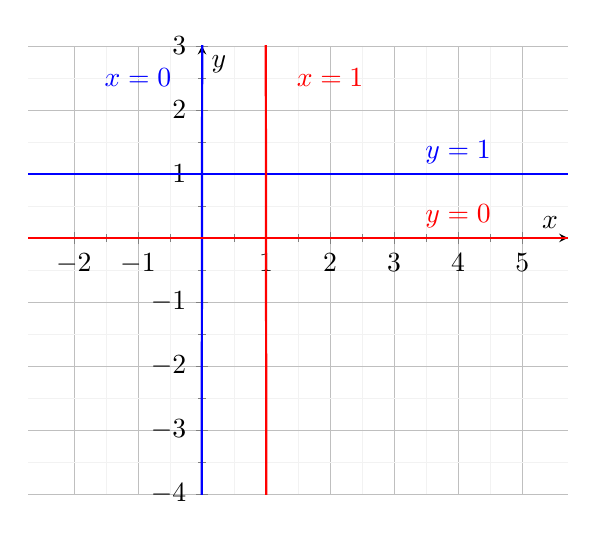
\begin{tikzpicture}
            \begin{axis}[
                axis lines=center,
                axis equal,
                xlabel=$x$, ylabel=$y$,
                xmin=-2, xmax=5,
                ymin=-4, ymax=3,
                xtick={-2,...,5},
                ytick={-4,...,3},
                grid=both,
                grid style={line width=.1pt, draw=gray!10},
                major grid style={line width=.2pt,draw=gray!50},
                minor tick num=1,
                clip=true
            ]
                
                % Recta x=0
                \addplot[blue,thick,domain=-0.1:0.1] {900*x};
                \node[blue] at (axis cs:-1,2.5) {$x=0$};

                % Recta y=1
                \addplot[blue,thick,domain=-3:6] {1};
                \node[blue, above] at (axis cs:4,1) {$y=1$};

                % Recta y=0
                \addplot[red,thick,domain=-3:6] {0};
                \node[red, above] at (axis cs:4,0) {$y=0$};

                % Recta vertical x=1
                \addplot[red,thick,domain=0.9:1.1] {-900*x+900};
                \node[red] at (axis cs:2,2.5) {$x=1$};
            \end{axis}
        \end{tikzpicture}
    \end{figure}

    \begin{description}
        \item[Opción 1:] Composición de un giro con una traslación.

        Sean las las siguientes rectas, con sus respectivas imágenes:
        \begin{gather*}
            r=(0,0)+\cc{L}\{(0,1)\} \longrightarrow f(r)=(1,1)+\cc{L}\{(-1,0)\} \\
            s=(0,0)+\cc{L}\{(1,0)\} \longrightarrow f(s)=(1,1)+\cc{L}\{(0,1)\}
        \end{gather*}

        Podemos ver que una posible solución es que $f$ sea la composición de un giro de 90 grados centrado en el origen junto con una traslación según el vector $(1,1)$.
        
        \item[Opción 2:] Simetría axial.

        También podemos ver las rectas, con sus respectivas imágenes, de la siguiente forma:
        \begin{gather*}
            r=(0,1)+\cc{L}\{(0,1)\} \longrightarrow f(r)=(0,1)+\cc{L}\{(-1,0)\} \\
            s=(1,0)+\cc{L}\{(1,0)\} \longrightarrow f(s)=(1,0)+\cc{L}\{(0,-1)\}
        \end{gather*}

        Podemos ver que hay dos puntos fijos, $(0,1), (1,0)$. Tenemos que se trata de la reflexión axial respecto de $L=(0,1)+\cc{L}\{(1,-1)\}$; es decir, $L\equiv y=-x+1$.
    \end{description}
\end{ejercicio}

\begin{ejercicio}
    Sean $f_1, f_2$ las simetrías (ortogonales) de $\bb{R}^2$ respecto de las rectas $R_1 = \{(x, y) \in \bb{R}^2 \mid x - y = 2\}$ y $R_2=\{(x, y) \in \bb{R}^2 \mid x - 2y = 1\}$, respectivamente. Calcula $f_1 \circ f_2$ y descríbela geométricamente.

    \begin{figure}[H]
        \centering
        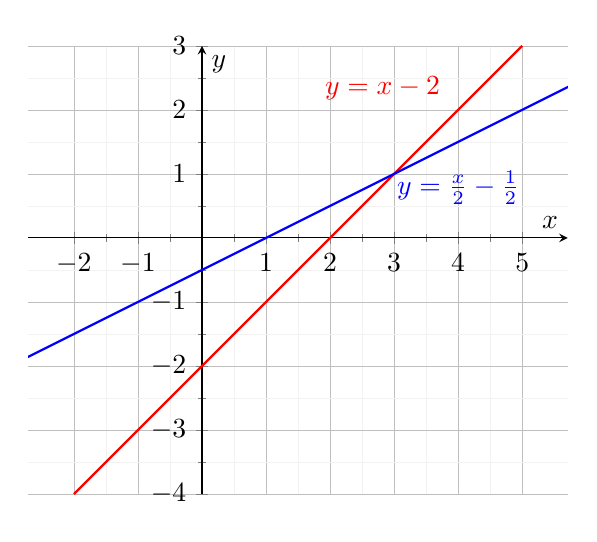
\begin{tikzpicture}
            \begin{axis}[
                axis lines=center,
                axis equal,
                xlabel=$x$, ylabel=$y$,
                xmin=-2, xmax=5,
                ymin=-4, ymax=3,
                xtick={-2,...,5},
                ytick={-4,...,3},
                grid=both,
                grid style={line width=.1pt, draw=gray!10},
                major grid style={line width=.2pt,draw=gray!50},
                minor tick num=1,
                clip=true
            ]
                \addplot[red,thick,domain=-2:5] {x-2};
                \addplot[blue,thick,domain=-3:6] {x/2-1/2};

                \node[red,above left, xshift=-3pt] at (axis cs:4,2) {$y=x-2$};
                \node[blue, yshift=-5pt] at (axis cs:4,1) {$y=\frac{x}{2}-\frac{1}{2}$};
            \end{axis}
        \end{tikzpicture}
    \end{figure}

    En primer lugar, como la composición de isometrías es una isometría, tenemos que $f_1\circ f_2$ es una isometría.
    Además, como $f_1,f_2$ son simetrías (movimientos inversos), tenemos que $|f_1\circ f_2| = |f_1||f_2| = 1$, por lo que se trata de un movimiento directo.
    Además, $p=(3,1)\in R_1\cap R_2$. Por lo que $p\in \cc{P}_{f_1\circ f_2}$.

    Tenemos que $R_1 = p+\cc{L}\{(1,1)\}$ y $R_2 = p+\cc{L}\{(2,1)\}$, por lo que:
    \begin{equation*}
        {R_1}_p^\perp = p+\cc{L}\{(1,-1)\} \qquad \qquad {R_2}_p^\perp = p+\cc{L}\{(2,-1)\}
    \end{equation*}

    Por tanto, sea $\cc{R}_1 = \{p, \cc{B}_1 = \{(1,1), (1,-1)\}\}$ y $\cc{R}_2 = \{p, \cc{B}_2 = \{(2,1), (-1,2)\}\}$ sistemas de referencia ortogonales de $\bb{R}^2$. Entonces, tenemos que:
    \begin{equation*}
        M(f_1,\cc{R}_1) = \left(\begin{array}{c|cc}
            1 & 0 & 0 \\ \hline
            0 & 1 & 0 \\
            0 & 0 & -1
        \end{array}\right)
        \qquad \qquad
        M(f_2,\cc{R}_2) = \left(\begin{array}{c|cc}
            1 & 0 & 0 \\ \hline
            0 & 1 & 0 \\
            0 & 0 & -1
        \end{array}\right)
    \end{equation*}

    Buscamos expresar las matrices de $f_1$ y $f_2$ en el sistema de referencia $\cc{R} = \{p, \cc{B}_u\}$.
    Tenemos que:
    \begin{align*}
        M(f_1,\cc{R}) &= M(Id_{\bb{R}^2},\cc{R}_1,\cc{R})\cdot M(f_1,\cc{R}_1) \cdot M(Id_{\bb{R}^2},\cc{R},\cc{R}_1) =\\
        &= \left(\begin{array}{c|cc}
            1 & 0 & 0 \\ \hline
            0 & 1 & 1 \\
            0 & 1 & -1
        \end{array}\right)
        \left(\begin{array}{c|cc}
            1 & 0 & 0 \\ \hline
            0 & 1 & 0 \\
            0 & 0 & -1
        \end{array}\right)
        \left(\begin{array}{c|cc}
            1 & 0 & 0 \\ \hline
            0 & 1 & 1 \\
            0 & 1 & -1
        \end{array}\right)^{-1}
        = \left(\begin{array}{c|cc}
            1 & 0 & 0 \\ \hline
            0 & 0 & 1 \\
            0 & 1 & 0
        \end{array}\right)
    \end{align*}
    \begin{align*}
        M(f_2,\cc{R}) &= M(Id_{\bb{R}^2},\cc{R}_2,\cc{R})\cdot M(f_2,\cc{R}_2) \cdot M(Id_{\bb{R}^2},\cc{R},\cc{R}_2) =\\
        &= \left(\begin{array}{c|cc}
            1 & 0 & 0 \\ \hline
            0 & 2 & -1 \\
            0 & 1 & 2
        \end{array}\right)
        \left(\begin{array}{c|cc}
            1 & 0 & 0 \\ \hline
            0 & 1 & 0 \\
            0 & 0 & -1
        \end{array}\right)
        \left(\begin{array}{c|cc}
            1 & 0 & 0 \\ \hline
            0 & 2 & -1 \\
            0 & 1 & 2
        \end{array}\right)^{-1}
        = \frac{1}{5}\left(\begin{array}{c|cc}
            5 & 0 & 0 \\ \hline
            0 & 3 & 4 \\
            0 & 4 & -3
        \end{array}\right)
    \end{align*}

    Por tanto, tenemos que:
    \begin{equation*}
        M(f_1\circ f_2,\cc{R}) = M(f_1,\cc{R})\cdot M(f_2,\cc{R})
        = \frac{1}{5}\left(\begin{array}{c|cc}
            5 & 0 & 0 \\ \hline
            0 & 4 & -3 \\
            0 & 3 & 4
        \end{array}\right)
    \end{equation*}

    Por tanto, tenemos que es un movimiento directo con puntos fijos en el plano. Como $f_1\circ f_2\neq Id_{\bb{R}^2}$, entonces se trata de
    un giro de centro su punto fijo, $p=(3,1)$. Para calcular el ángulo no orientado, sabemos que el ángulo de giro cumple que:
    \begin{equation*}
        2\cos \theta = {tr\left(M\left(\vec{f_1\circ f_2},\cc{B}_u\right)\right)} = \frac{8}{5} \Longrightarrow \theta = \arccos \left(\frac{4}{5}\right) \approx 0.64 \text{ rad}
    \end{equation*}
\end{ejercicio}

\begin{ejercicio}
    Considera un espacio afín euclídeo $\bb{E}$ de dimensión 3, y sea $f$ un movimiento rígido de $\bb{E}$ tal que $f(1, 0, 1) = (2, -3, 1)$ en coordenadas de un sistema de referencia euclídeo fijo. Si sabemos que $f$ es la simetría respecto de un plano, calcula dicho plano.\\

    Consideramos en primer lugar el punto medio entre $p=(1,0,1)$ y su imagen $f(p)=(2,-3,1)$, $m_{pf(p)} = \left(\nicefrac{3}{2},\nicefrac{-3}{2},1\right)$.
    Por tanto, el plano buscado es el que pasa por $m_{pf(p)}$ y es perpendicular a $\vec{pf(p)}$; es decir, $\pi = m_{pf(p)} + \cc{L}\{\vec{pf(p)}\}^\perp$.

    Buscamos ahora los vectores directores del plano. Tenemos que $\vec{pf(p)} = (1,-3,0)$ es ortogonal al plano, por lo que
    buscamos dos vectores perpendiculares a él. Como $(0,0,1)$ y $(3,1, 0)$ son ortogonales a $\vec{pf(p)}$ y los tres vectores forman base de $\bb{R}^3$,
    entonces $\cc{L}\{\vec{pf(p)}\}^\perp = \cc{L}\{(0,0,1), (3,1,0)\}$. Por tanto, el plano buscado es:
    \begin{equation*}
        \pi = \left(\frac{3}{2},\frac{-3}{2},1\right) + \cc{L}\{(0,0,1), (3,1,0)\}
    \end{equation*}
\end{ejercicio}

\begin{ejercicio}
    Sea $\cc{A}$ un espacio afín euclídeo de dimensión 2, y sean $R_1$ y $R_2$ dos rectas de $\cc{A}$.
    Prueba que siempre es posible encontrar un movimiento rígido $f : \cc{A} \to \cc{A}$ que lleve $R_1$ en $R_2$.
    Estudia de qué tipo es $f$, según la posición relativa de $R_1$ y $R_2$. ¿Se puede elegir siempre directo? ¿E inverso?\\

    Hay tres opciones, según la posición relativa de $R_1$ y $R_2$:
    \begin{enumerate}
        \item $R_1\cap R_2 = R_1 = R_2$. Es decir, las rectas son coincidentes.
        
        En este caso, hay muchas posibilidades. El caso más sencillo es que $f=Id_{\cc{A}}$, siendo $f$ un movimiento directo.
        También puede ser la simetría respecto de $R_1$, siendo $f$ un movimiento inverso.

        \item $R_1\cap R_2 = \emptyset$. Es decir, las rectas son paralelas.
        
        \begin{figure}[H]
            \centering
            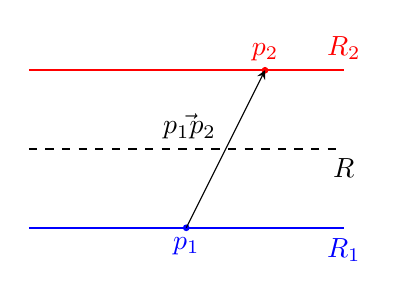
\begin{tikzpicture}
                % Recta R1
                \draw[blue, thick] (-2,0) -- (2,0) node[below] {$R_1$};
                % Recta R2
                \draw[red, thick] (-2,2) -- (2,2) node[above] {$R_2$};

                % Punto p_1 \in R1
                \filldraw[blue] (0,0) circle (1pt) node[below] {$p_1$};
                % Punto p_2 \in R2
                \filldraw[red] (1,2) circle (1pt) node[above] {$p_2$};
                % Vector de p_1 a p_2
                \draw[-stealth] (0,0) -- (1,2) node[midway, above left] {$\vec{p_1p_2}$};

                % Recta entre R1 y R2
                \draw[dashed] (-2,1) -- (2,1) node[below] {$R$};
            \end{tikzpicture}
            \caption{Distintas opciones en el caso de que $R_1\cap R_2 = \emptyset$.}
        \end{figure}

        En este caso tenemos que no hay puntos fijos.

        Sea $p_1\in R_1$ y $p_2\in R_2$. Entonces, el caso más sencillo es $f=t_{\vec{p_1p_2}}$, siendo $f$ un movimiento directo. Tenemos que:
        \begin{equation*}
            f(R_1) = t_{\vec{p_1p_2}}\left(p_1 + \vec{R_1}\right) = p_2 + \vec{R_1} = R_2
        \end{equation*}

        También puede ser la simetría respecto de la recta $R$, recta que se encuentra entre $R_1$ y $R_2$ (movimiento inverso). Si $p=m_{p_1p_2}$, entonces $R=p+\vec{R_1}$.


        \item $R_1\cap R_2 = \{p\}$. Es decir, las rectas son secantes.
        \begin{figure}[H]
            \centering
            \begin{tikzpicture}[scale=0.6]
                % Define los puntos de las rectas
                \coordinate (r1_ini) at (-4,-2);
                \coordinate (r1_fin) at (4,2);
                \coordinate (r2_ini) at (-4,2);
                \coordinate (r2_fin) at (4,-2);
    
                \coordinate (O) at (0,0);
                \coordinate (v_1) at (2,1);
                \coordinate (v_2) at (2,-1);
            
                % Dibuja las rectas
                \draw (r1_ini) -- (r1_fin);
                \draw (r2_ini) -- (r2_fin);
    
                % Etiqueta las rectas
                \node[right] at (r1_fin) {$R_1$};
                \node[right] at (r2_fin) {$R_2$};
    
                % Dibuja los vectores directores
                \draw[-stealth, blue] (O) -- node[above]{$v_1$} (v_1);
                \draw[-stealth, red] (O) -- node[below]{$v_2$} (v_2);
    
                \tkzMarkAngle[size=0.5](v_2,O,v_1);
                \tkzLabelAngle[pos=0.8](v_2,O,v_1){$\alpha$};

                % Punto de intersección
                \filldraw[black] (O) circle (2pt) node[above left] {$p$};

                % Recta entre R1 y R2
                \draw[dashed] (-4,0) -- (4,0) node[below] {$R$};
                \draw[dashed] (0,2) -- (0,-2) node[below] {$R'$};
            \end{tikzpicture}
            \caption{Distintas opciones en el caso de que $R_1\cap R_2=\{p\}$.}
        \end{figure}

        En este caso, como movimiento directo, la única opción es el giro de centro $p$ y ángulo orientado $\alpha=\measuredangle_o (R_1,R_2)$.

        Como movimientos inversos, podemos considerar cualquiera de la simetría respecto de cualquiera de las dos bisectrices entre $R_1$ y $R_2$ (estas son, en el dibujo, $R$ y $R'$).
    \end{enumerate}
    Por tanto, siempre se puede elegir una isometría directa y otra inversa que lleve $R_1$ en $R_2$.
\end{ejercicio}

\begin{ejercicio}
    Sea $\bb{E}$ un espacio afín euclídeo, y sean $p,q\in \bb{E}$, con $p\neq q$.
    Demuestra que existe una única simetría $\sigma_H$ respecto de un hiperplano $H\subset \bb{E}$ tal que $\sigma_H(p)=q$.

    Sea el vector $\vec{pq}$. Entonces, el hiperplano buscado es el que pasa por $m_{pq}$ y es perpendicular a $\vec{pq}$;
    es decir, $H = m_{pq} + \cc{L}\{\vec{pq}\}^\perp$.

    Efectivamente, tenemos que:
    \begin{equation*}
        \sigma_H(p) = \sigma_H\left(m_{pq} + \frac{1}{2}\vec{qp}\right) = m_{pq} - \frac{1}{2}\vec{qp} = q
    \end{equation*}

    Veamos ahora que es única. Supongamos que existe otro hiperplano $H'$ tal que $\sigma_{H'}(p)=q$. Veamos que $H=H'$.
    Como $\sigma_{H'}(p)=q$, tenemos que $m_{pq}=\pi_{H'}(p)$, por lo que $\vec{p~m_{pq}}\perp \vec{H'}$ y $m_{pq}\in H'$.
    No obstante, $\vec{p~m_{pq}}=\frac{1}{2}\vec{pq}$, por lo que $\vec{pq}\perp \vec{H'}$, y por tanto $\vec{pq}\in \vec{H'}^\perp$.
    Como $H'$ es un hiperplano, entonces $\vec{H'}^\perp = \cc{L}\{\vec{pq}\}^\perp$. Por tanto, $H'= m_{pq} + \cc{L}\{\vec{pq}\}^\perp = H$.
\end{ejercicio}

\begin{ejercicio}
    Sean $R_1$ y $R_2$ dos rectas que se cruzan en un espacio afín euclídeo tridimensional $\bb{E}$.
    Demuestra que existe una única recta afín $R$ que interseca de manera ortogonal a $R_1$ y $R_2$.
    Prueba además que la distancia de $R_1$ a $R_2$ es exactamente la distancia entre los puntos dados por $R_1 \cap R$ y $R_2 \cap R$.

    Sea $R_1=p_1 + \cc{L}\{v_1\}$ y $R_2=p_2 + \cc{L}\{v_2\}$.
    En el Teorema \ref{teo:existencia_vector_ortogonal}, hemos visto que existen $q_1\in R_1$ y $q_2\in R_2$
    tales que $\vec{q_1q_2}\perp \vec{R_1}$ y $\vec{q_1q_2}\perp \vec{R_2}$. Además, como $\vec{R_1}\cap \vec{R_2}=\{0\}$, tenemos que dichos puntos son únicos.

    Por tanto, la recta buscada es $R=q_1 + \cc{L}\{\vec{q_1q_2}\} = q_2 + \cc{L}\{\vec{q_1q_2}\}$.

    En el corolario de dicho Teorema, el Corolario \ref{coro:dist_ortogonal}, se vio que $d(R_1,R_2) = d(q_1,q_2)$.
\end{ejercicio}

\begin{ejercicio}
    Consideremos la aplicación $f : \bb{R}^2 \to \bb{R}^2$ que viene dada por $f(x, y) = (y -2, x+ 1)$.
    ¿Es $f$ un movimiento rígido? En tal caso, clasifícalo.

    Tenemos que:
    \begin{equation*}
        M(f,\cc{R}_0) = \left(
        \begin{array}{c|cc}
            1 & 0 & 0 \\ \hline
            -2 & 0 & 1 \\
            1 & 1 & 0 \\
        \end{array}
        \right)
    \end{equation*}

    Como $\cc{R}_0$ es un sistema de referencia ortonormal, para ver si $f$ es una isometría (equivalentemente vemos que $\vec{f}$ lo es) basta con probar que
    $M\left(\vec{f}, \cc{B}_u\right)\in~O(2)$. Tenemos que:
    \begin{equation*}
        M\left(\vec{f},\cc{B}_u\right)M\left(\vec{f},\cc{B}_u\right)^t
        = 
        \left(
        \begin{array}{cc}
            0 & 1 \\
            1 & 0 \\
        \end{array}
        \right)
        \left(
        \begin{array}{cc}
            0 & 1 \\
            1 & 0 \\
        \end{array}
        \right)
        = 
        \left(
        \begin{array}{cc}
            1 & 0 \\
            0 & 1 \\
        \end{array}
        \right) = Id_2
    \end{equation*}

    Por tanto, $f$ es una isometría. Como $\left|\vec{f}\right|=-1$, tenemos que $f$ es una isometría inversa en el plano. Calculemos sus puntos fijos:
    \begin{equation*}
        \left(
        \begin{array}{c|cc}
            1 & 0 & 0 \\ \hline
            -2 & 0 & 1 \\
            1 & 1 & 0 \\
        \end{array}
        \right)
        \left(
        \begin{array}{c}
            1\\x\\y
        \end{array}
        \right)
        =\left(
            \begin{array}{c}
                1\\x\\y
            \end{array}
        \right)
    \end{equation*}

    Equivalentemente, tenemos que:
    \begin{equation*}
        \left(
        \begin{array}{cc}
            -1 & 1 \\
            1 & -1 \\
        \end{array}
        \right)
        \left(
        \begin{array}{c}
            x\\y
        \end{array}
        \right)
        =\left(
            \begin{array}{c}
                2 \\ -1
            \end{array}
        \right)
    \end{equation*}

    Por tanto, no hay puntos fijos, por lo que se trata de una simetría axial con desplazamiento. Calculemos en primer lugar el eje de simetría, $\vec{L}$.
    Como $\vec{f}= \sigma_{\vec{L}}$, tenemos que $\vec{L}=V_1$:
    \begin{align*}
        \vec{L}&= \left\{(x,y)\in \bb{R}^2 \mid \left(M\left(\vec{f}, \cc{B}_u\right) - Id\right)(x,y)^t = 0\right\} =\\
        &= \left\{(x,y)\in \bb{R}^2 \mid \left(
        \begin{array}{cc}
            -1 & 1 \\
            1 & -1 \\
        \end{array}
        \right)
        \left(
        \begin{array}{c}
            x\\y
        \end{array}
        \right)
        =\left(
            \begin{array}{c}
                0 \\ 0
            \end{array}
        \right)\right\} = \cc{L}\{(1,1)\}
    \end{align*}

    Calculamos ahora un punto de $\vec{L}$. Tenemos que $m_{p f(p)}\in L$ para todo $p\in \bb{R}^2$. En particular, para $p=(0,0)$, tenemos que $f(p)=(-2,1)$, por lo que:
    \begin{equation*}
        m_{0 f(0)} = \left(\frac{-2}{2},\frac{1}{2}\right) = \left(-1, \frac{1}{2}\right) \in L
    \end{equation*}

    Por tanto, tenemos que el eje de la simetría es:
    \begin{equation*}
        L = \left(-1, \frac{1}{2}\right) + \cc{L}\{(1,1)\}
    \end{equation*}

    Por último, calculamos el desplazamiento. Para ello, tomamos un punto cualquiera de $L$, por ejemplo, $p=\left(-1, \frac{1}{2}\right)$, y tenemos que $f(p)=(\nicefrac{-3}{2}, 0)$.
    Por tanto, el vector de desplazamiento es:
    \begin{equation*}
        \vec{v} = \vec{p f(p)} = \left(\frac{-3}{2} - (-1), 0 - \frac{1}{2}\right) = \left(-\frac{1}{2}, -\frac{1}{2}\right) = -\frac{1}{2}(1,1)
    \end{equation*}
\end{ejercicio}

\begin{ejercicio}
    Demostrar que si $p$ y $q$ son dos puntos de un espacio afín euclídeo $\bb{E}$, entonces siempre existe un movimiento rígido
    $f : \bb{E} \to \bb{E}$ tal que $f(p) = q$. De forma más general, probar que si $\bb{E}$ tiene dimensión finita y
    $S$, $S'$ son dos subespacios afines de $\bb{E}$ de dimensión $m$, entonces existe un movimiento rígido $f : \bb{E} \to \bb{E}$ tal que $f(S) = S'$.\\

    Dados dos puntos $p,q\in \bb{E}$, consideramos el vector $\vec{pq}$. Entonces, el movimiento buscado es la traslación según el vector $\vec{pq}$, ya que:
    \begin{equation*}
        t_{\vec{pq}}(p) = p + \vec{pq} = q
    \end{equation*}

    En el caso general, si $S=p+\cc{L}\{v_1,\dots,v_m\}$ y $S'=p'+\cc{L}\{v'_1,\dots,v'_m\}$, ambas bases ortonormales, entonces buscamos un movimiento rígido
    $f$ tal que $f(p)=p'$ y $\vec{f}(v_i)=v'_i$ para todo $i=1,\dots,m$.

    Consideramos los siguientes sistemas de referencia euclídeos:
    \begin{align*}
        \cc{R} &= \{p, \cc{B} = \{v_1,\dots,v_m, v_{m+1}, \dots, v_n\}\}\\
        \cc{R}' &= \{p', \cc{B}' = \{v'_1,\dots,v'_m, v'_{m+1}, \dots, v'_n\}\}
    \end{align*}
    donde $v_i, v'_i$ para $i=m+1,\dots,n$ son vectores ortonormales que completan las bases $\cc{B}, \cc{B}'$ respectivamente.
    Entonces, sea la aplicación $f : \bb{E} \to \bb{E}$ cuya matriz asociada en dichos sistemas de referencia es:
    \begin{equation*}
        M(\vec{f},\cc{R},\cc{R}') = \left(
        \begin{array}{c|c}
            1 & 0 \\ \hline
            0 & Id_n
        \end{array}
        \right)
    \end{equation*}
    
    Tenemos que $f(p) = f(0_{\cc{R}}) = 0_{\cc{R}'} = p'$. Además, $\vec{f}\left(\vec{S}\right)=\vec{S'}$, y por tanto tenemos que $f(S)=S'$, como queríamos demostrar.
\end{ejercicio}

\begin{ejercicio}
    Consideremos la aplicación $f : \bb{R}^2 \to \bb{R}^2$ que viene dada por $f(x, y) = (2y - 1, -2x + 3)$. ¿Es $f$ un movimiento rígido? En tal caso, clasifícalo.

    Tenemos que:
    \begin{equation*}
        M(f,\cc{R}_0) = \left(
        \begin{array}{c|cc}
            1 & 0 & 0 \\ \hline
            -1 & 0 & 2 \\
            3 & -2 & 0 \\
        \end{array}
        \right)
    \end{equation*}

    Como $\cc{R}_0$ es un sistema de referencia ortonormal, para ver si $f$ es una isometría (equivalentemente vemos que $\vec{f}$ lo es) basta con probar que
    $M\left(\vec{f}, \cc{B}_u\right)\in~O(2)$. Como $\left|\vec{f}\right|=4\neq \pm 1$, tenemos que $f$ no es una isometría.
\end{ejercicio}

\begin{ejercicio}
    Sean $f_1, f_2 : \bb{R}^2\to \bb{R}^2$ las isometrías dadas, respectivamente, por las simetrías respecto de las rectas de ecuación $x + y = 0$ y $x + 2y = 2$.
    \begin{figure}[H]
        \centering
        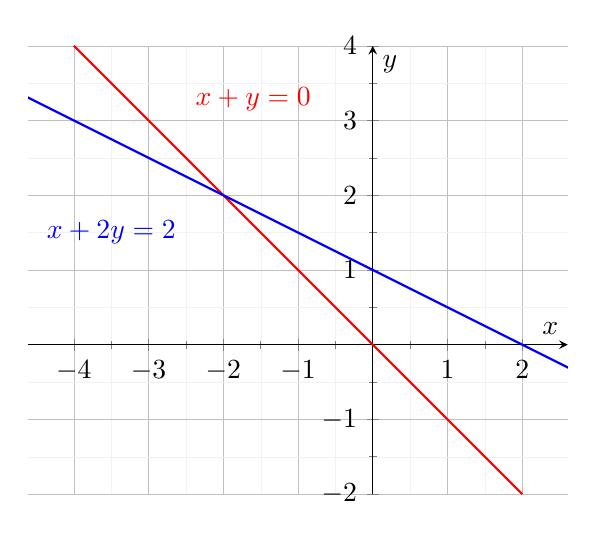
\begin{tikzpicture}
            \begin{axis}[
                axis lines=center,
                axis equal,
                xlabel=$x$, ylabel=$y$,
                xmin=-4, xmax=2,
                ymin=-2, ymax=4,
                xtick={-4,...,2},
                ytick={-2,...,4},
                grid=both,
                grid style={line width=.1pt, draw=gray!10},
                major grid style={line width=.2pt,draw=gray!50},
                minor tick num=1,
                clip=true
            ]
                \addplot[red,thick,domain=-4:2] {-x};
                \addplot[blue,thick,domain=-5:3] {-x/2+1};

                \node[red, above right] at (axis cs:-2.5,3) {$x+y=0$};
                \node[blue] at (axis cs:-3.5,1.5) {$x+2y=2$};
            \end{axis}
        \end{tikzpicture}
    \end{figure}
    \begin{enumerate}
        \item Calcula explícitamente $f_1$ y $f_2$ en coordenadas usuales.
        
        Sea $R_1=\{(x,y)\in \bb{R}^2 \mid x+y=0\}$ y $R_2=\{(x,y)\in \bb{R}^2 \mid x+2y=2\}$.

        Tenemos que $R_1 = (-2,2) + \cc{L}\{(1,-1)\}$ y $R_2 = (-2,2) + \cc{L}\{(2,-1)\}$, por lo que:
        \begin{equation*}
            {R_1}_{(-2,2)}^\perp = (-2,2) + \cc{L}\{(1,1)\} \qquad \qquad {R_2}_{(-2,2)}^\perp = (-2,2) + \cc{L}\{(1, 2)\}
        \end{equation*}

        Por tanto, sea $\cc{R}_1 = \{(-2,2), \cc{B}_1 = \{(1,-1), (1,1)\}\}$ y $\cc{R}_2 = \{(-2,2), \cc{B}_2 = \{(2,-1), (1,2)\}\}$ sistemas de referencia ortogonales de $\bb{R}^2$. Entonces, tenemos que:
        \begin{equation*}
            M(f_1,\cc{R}_1) = \left(\begin{array}{c|cc}
                1 & 0 & 0 \\ \hline
                0 & 1 & 0 \\
                0 & 0 & -1
            \end{array}\right) = M(f_2,\cc{R}_2)
        \end{equation*}

        Para calcular las matrices de $f_1$ y $f_2$ en el sistema de referencia $\cc{R}_0 = \{(0,0), \cc{B}_u\}$, tenemos:
        \begin{align*}
            M(f_1,\cc{R}_0) &= M(Id_{\bb{R}^2},\cc{R}_1,\cc{R}_0)\cdot M(f_1,\cc{R}_1) \cdot M(Id_{\bb{R}^2},\cc{R}_0,\cc{R}_1) =\\
            &= \left(\begin{array}{c|cc}
                1 & 0 & 0 \\ \hline
                -2 & 1 & 1 \\
                2 & -1 & 1
            \end{array}\right)
            \left(\begin{array}{c|cc}
                1 & 0 & 0 \\ \hline
                0 & 1 & 0 \\
                0 & 0 & -1
            \end{array}\right)
            \left(\begin{array}{c|cc}
                1 & 0 & 0 \\ \hline
                -2 & 1 & 1 \\
                2 & -1 & 1
            \end{array}\right)^{-1}
            =\\&= \left(\begin{array}{c|cc}
                1 & 0 & 0 \\ \hline
                0 & 0 & -1 \\
                0 & -1 & 0
            \end{array}\right)
        \end{align*}

        \begin{align*}
            M(f_2,\cc{R}_0) &= M(Id_{\bb{R}^2},\cc{R}_2,\cc{R}_0)\cdot M(f_2,\cc{R}_2) \cdot M(Id_{\bb{R}^2},\cc{R}_0,\cc{R}_2) =\\
            &= \left(\begin{array}{c|cc}
                1 & 0 & 0 \\ \hline
                -2 & 2 & 1 \\
                2 & -1 & 2
            \end{array}\right)
            \left(\begin{array}{c|cc}
                1 & 0 & 0 \\ \hline
                0 & 1 & 0 \\
                0 & 0 & -1
            \end{array}\right)
            \left(\begin{array}{c|cc}
                1 & 0 & 0 \\ \hline
                -2 & 2 & 1 \\
                2 & -1 & 2
            \end{array}\right)^{-1}
            =\\&= \frac{1}{5}\left(\begin{array}{c|cc}
                5 & 0 & 0 \\ \hline
                4 & 3 & -4 \\
                8 & -4 & -3
            \end{array}\right)
        \end{align*}

        \item Clasifica el movimiento rígido $g = f_1 \circ f_2$.
        
        En primer lugar, como la composición de isometrías es una isometría, tenemos que $g=f_1\circ f_2$ es una isometría. Por tanto:
        \begin{equation*}
            M(g,\cc{R}_0) = M(f_1\circ f_2,\cc{R}_0) = M(f_1,\cc{R}_0)\cdot M(f_2,\cc{R}_0)
            = \frac{1}{5}\left(\begin{array}{c|cc}
                5 & 0 & 0 \\ \hline
                -8 & 4 & 3 \\
                -4 & -3 & 4
            \end{array}\right)
        \end{equation*}

        Además, como $|g|=|f_1\circ f_2| = |f_1|\cdot |f_2| = 1$, tenemos que $g$ es una isometría directa en el plano. Además, como
        $(-2,2) \in R_1\cap R_2$, tenemos que $(-2,2)\in \cc{P}_g$, por lo que $g$ es un movimiento directo con puntos fijos en el plano.
        Como $g\neq Id_{\bb{R}^2}$, entonces se trata de un giro de centro su punto fijo, $p=(-2,2)$. Para calcular el ángulo no orientado, sabemos que el ángulo de giro cumple que:
        \begin{equation*}
            2\cos \theta = {tr\left(M\left(\vec{g},\cc{B}_u\right)\right)} = \frac{1}{5}(4+4) = \frac{8}{5} \Longrightarrow \theta = \arccos \left(\frac{4}{5}\right) \approx 0.64 \text{ rad}
        \end{equation*}
    \end{enumerate}
\end{ejercicio}

\begin{ejercicio}
    Demuestra que las siguientes aplicaciones son movimientos rígidos del plano y clasifícalos.
    \begin{enumerate}
        \item $f\left(x, y\right) = \left(3 - \dfrac{3x}{5} + \dfrac{4y}{5}, 1 - \dfrac{4x}{5} - \dfrac{3y}{5}\right).$

        Tenemos que:
        \begin{equation*}
            M(f,\cc{R}_0) = \left(
            \begin{array}{c|cc}
                1 & 0 & 0 \\ \hline
                3 & \nicefrac{-3}{5} & \nicefrac{4}{5} \\
                1 & \nicefrac{-4}{5} & \nicefrac{-3}{5} \\
            \end{array}
            \right)
        \end{equation*}

        Como $\cc{R}_0$ es un sistema de referencia ortonormal, para ver si $f$ es una isometría (equivalentemente vemos que $\vec{f}$ lo es) basta con probar que $M\left(\vec{f}, \cc{B}_u\right)\in~O(2)$. Tenemos que:
        \begin{equation*}
            M\left(\vec{f},\cc{B}_u\right)M\left(\vec{f},\cc{B}_u\right)^t
            = 
            \left(
            \begin{array}{cc}
                \nicefrac{-3}{5} & \nicefrac{4}{5} \\
                \nicefrac{-4}{5} & \nicefrac{-3}{5} \\
            \end{array}
            \right)
            \left(
            \begin{array}{cc}
                \nicefrac{-3}{5} & \nicefrac{-4}{5} \\
                \nicefrac{4}{5} & \nicefrac{-3}{5} \\
            \end{array}
            \right)
            = 
            \left(
            \begin{array}{cc}
                1 & 0 \\
                0 & 1 \\
            \end{array}
            \right) = Id_2
        \end{equation*}
        Por tanto, $\vec{f}$ es una isometría y por tanto, también lo es $f$. Como $|f|=1$, tenemos que $f$ es una isometría directa en el plano. Calculamos sus puntos fijos $(x,y)\in \bb{R}^2$:
        \begin{equation*}
            \left(
            \begin{array}{cc}
                \nicefrac{-3}{5}-1 & \nicefrac{4}{5} \\
                \nicefrac{-4}{5} & \nicefrac{-3}{5}-1 \\
            \end{array}
            \right)
            \left(
            \begin{array}{c}
                x\\y
            \end{array}
            \right)
            =\left(
            \begin{array}{cc}
                \nicefrac{-8}{5} & \nicefrac{4}{5} \\
                \nicefrac{-4}{5} & \nicefrac{-8}{5} \\
            \end{array}
            \right)
            \left(
            \begin{array}{c}
                x\\y
            \end{array}
            \right)
            = \left(
            \begin{array}{c}
                -3\\-1
            \end{array}
            \right)
        \end{equation*}

        Equivalentemente,
        \begin{equation*}
            \left(
            \begin{array}{cc}
                -8 & 4 \\
                -4 & -8 \\
            \end{array}
            \right)
            \left(
            \begin{array}{c}
                x\\y
            \end{array}
            \right)
            = \left(
            \begin{array}{c}
                -15\\-5
            \end{array}
            \right)
        \end{equation*}

        Por tanto, tenemos que solo hay un punto fijo, el punto $o=\frac{1}{4}(7,-1)$. Por tanto, se traza de un giro en el plano centrado en el punto $o$. Para calcular el ángulo no orientado sabemos que:
        \begin{equation*}
            2\cos\theta = tr\left(M\left(\vec{f}, \cc{B}_u\right)\right) = -\frac{6}{5} \Longrightarrow \cos\theta = -\frac{6}{10} = -\frac{3}{5} \Longrightarrow \theta \approx 2.21\text{ rad}
        \end{equation*}

        Por tanto, se trata de un giro en el plano centrado en el punto $o=\frac{1}{4}(7,-1)$ y de ángulo $\theta \approx 2.21\text{ rad}$.

        
        
        \item $f\left(x, y\right) = \left(\dfrac{x}{2} -\dfrac{\sqrt{3} y}{2} + 1,\dfrac{\sqrt{3} x}{2}+ \dfrac{y}{2} + 2\right).$

        Tenemos que:
        \begin{equation*}
            M(f,\cc{R}_0) = \left(
            \begin{array}{c|cc}
                1 & 0 & 0 \\ \hline
                1 & \nicefrac{1}{2} & \nicefrac{-\sqrt{3}}{2} \\
                2 & \nicefrac{\sqrt{3}}{2} & \nicefrac{1}{2} \\
            \end{array}
            \right)
        \end{equation*}

        Como $\cc{R}_0$ es un sistema de referencia ortonormal, para ver si $f$ es una isometría (equivalentemente vemos que $\vec{f}$ lo es) basta con probar que $M\left(\vec{f}, \cc{B}_u\right)\in~O(2)$. Tenemos que:
        \begin{equation*}
            M\left(\vec{f},\cc{B}_u\right)M\left(\vec{f},\cc{B}_u\right)^t
            = 
            \left(
            \begin{array}{cc}
                \nicefrac{1}{2} & \nicefrac{-\sqrt{3}}{2} \\
                \nicefrac{\sqrt{3}}{2} & \nicefrac{1}{2}
            \end{array}
            \right)
            \left(
            \begin{array}{cc}
                \nicefrac{1}{2} & \nicefrac{\sqrt{3}}{2} \\
                \nicefrac{-\sqrt{3}}{2} & \nicefrac{1}{2}
            \end{array}
            \right)
            = 
            \left(
            \begin{array}{cc}
                1 & 0 \\
                0 & 1 \\
            \end{array}
            \right) = Id_2
        \end{equation*}
        Por tanto, $\vec{f}$ es una isometría y por tanto, también lo es $f$. Como $|f|=1$, tenemos que $f$ es una isometría directa en el plano. Calculamos sus puntos fijos $(x,y)\in \bb{R}^2$:
        \begin{equation*}
            \left(
            \begin{array}{cc}
                \nicefrac{1}{2}-1 & \nicefrac{-\sqrt{3}}{2} \\
                \nicefrac{\sqrt{3}}{2} & \nicefrac{1}{2}-1
            \end{array}
            \right)
            \left(
            \begin{array}{c}
                x\\y
            \end{array}
            \right)
            =\left(
            \begin{array}{cc}
                \nicefrac{-1}{2} & \nicefrac{-\sqrt{3}}{2} \\
                \nicefrac{\sqrt{3}}{2} & \nicefrac{-1}{2}
            \end{array}
            \right)
            \left(
            \begin{array}{c}
                x\\y
            \end{array}
            \right)
            = \left(
            \begin{array}{c}
                -1\\-2
            \end{array}
            \right)
        \end{equation*}

        Equivalentemente,
        \begin{equation*}
            \left(
            \begin{array}{cc}
                -1 & -\sqrt{3} \\
                \sqrt{3} & -1 \\
            \end{array}
            \right)
            \left(
            \begin{array}{c}
                x\\y
            \end{array}
            \right)
            = \left(
            \begin{array}{c}
                -2\\-4
            \end{array}
            \right)
        \end{equation*}

        Por tanto, tenemos que solo hay un punto fijo, el punto $$o=\frac{1}{2}(-2\sqrt{3}+1,\sqrt{3}+2)$$ Por tanto, se traza de un giro en el plano centrado en el punto $o$. Para calcular el ángulo no orientado sabemos que:
        \begin{equation*}
            2\cos\theta = tr\left(M\left(\vec{f}, \cc{B}_u\right)\right) = 1 \Longrightarrow \cos\theta = \frac{1}{2} \Longrightarrow \theta =\frac{\pi}{3}\text{ rad}
        \end{equation*}

        Por tanto, se trata de un giro en el plano de ángulo $\theta =\frac{\pi}{3}\text{ rad}$ y centrado en el punto $o=\frac{1}{2}(-2\sqrt{3}+1,\sqrt{3}+2)$.


        
        \item $f\left(x, y\right) = \left(-\dfrac{x}{2} + \dfrac{\sqrt{3}y}{2} + 1,\dfrac{\sqrt{3} x}{2} + \dfrac{y}{2} - 1\right).$

        Tenemos que:
        \begin{equation*}
            M(f,\cc{R}_0) = \left(
            \begin{array}{c|cc}
                1 & 0 & 0 \\ \hline
                1 & \nicefrac{-1}{2} & \nicefrac{\sqrt{3}}{2} \\
                -1 & \nicefrac{\sqrt{3}}{2} & \nicefrac{1}{2} \\
            \end{array}
            \right)
        \end{equation*}

        Como $\cc{R}_0$ es un sistema de referencia ortonormal, para ver si $f$ es una isometría (equivalentemente vemos que $\vec{f}$ lo es) basta con probar que $M\left(\vec{f}, \cc{B}_u\right)\in~O(2)$. Tenemos que:
        \begin{equation*}
            M\left(\vec{f},\cc{B}_u\right)M\left(\vec{f},\cc{B}_u\right)^t
            = 
            \left(
            \begin{array}{cc}
                \nicefrac{-1}{2} & \nicefrac{\sqrt{3}}{2} \\
                \nicefrac{\sqrt{3}}{2} & \nicefrac{1}{2}
            \end{array}
            \right)
            \left(
            \begin{array}{cc}
                \nicefrac{-1}{2} & \nicefrac{\sqrt{3}}{2} \\
                \nicefrac{\sqrt{3}}{2} & \nicefrac{1}{2}
            \end{array}
            \right)
            = 
            \left(
            \begin{array}{cc}
                1 & 0 \\
                0 & 1 \\
            \end{array}
            \right) = Id_2
        \end{equation*}
        Por tanto, $\vec{f}$ es una isometría y por tanto, también lo es $f$. Como $|f|=-1$, tenemos que $f$ es una isometría inversa en el plano. Calculamos sus puntos fijos $(x,y)\in \bb{R}^2$:
        \begin{equation*}
            \left(
            \begin{array}{cc}
                \nicefrac{-1}{2}-1 & \nicefrac{\sqrt{3}}{2} \\
                \nicefrac{\sqrt{3}}{2} & \nicefrac{1}{2}-1
            \end{array}
            \right)
            \left(
            \begin{array}{c}
                x\\y
            \end{array}
            \right)
            =\left(
            \begin{array}{cc}
                \nicefrac{-3}{2} & \nicefrac{\sqrt{3}}{2} \\
                \nicefrac{\sqrt{3}}{2} & \nicefrac{-1}{2}
            \end{array}
            \right)
            \left(
            \begin{array}{c}
                x\\y
            \end{array}
            \right)
            = \left(
            \begin{array}{c}
                -1\\1
            \end{array}
            \right)
        \end{equation*}

        Equivalentemente,
        \begin{equation*}
            \left(
            \begin{array}{cc}
                -3 & \sqrt{3} \\
                \sqrt{3} & -1 \\
            \end{array}
            \right)
            \left(
            \begin{array}{c}
                x\\y
            \end{array}
            \right)
            = \left(
            \begin{array}{c}
                -2\\2
            \end{array}
            \right)
        \end{equation*}

        Por tanto, tenemos que $f$ no tiene puntos fijos, ya que ese sistema es un SI. Por tanto, tenemos que es una simetría axial con deslizamiento.

        Calculamos en primer lugar su eje de simetría $L$, buscando primero $\vec{L}$. Como $\vec{f}=\sigma_{\vec{L}}$, tenemos que $\vec{L}=V_1$, por lo que:
        \begin{equation*}
            \begin{split}
                \vec{L} &= \{ (x,y)\in \bb{R}^2 \mid (M\left(\vec{f}, \cc{B}_u\right) - Id) (x,y)^t = (0,0)^t \} =\\
                &= \left\{ (x,y)\in \bb{R}^2 \mid \left(
                \begin{array}{cc}
                    \nicefrac{-1}{2}-1 & \nicefrac{\sqrt{3}}{2} \\
                    \nicefrac{\sqrt{3}}{2} & \nicefrac{1}{2}-1
                \end{array}
                \right)
                \left(
                \begin{array}{c}
                    x\\y
                \end{array}
                \right)
                = \left(
                \begin{array}{c}
                    0\\0
                \end{array}
                \right)
                \right\} =\\
                &= \left\{ (x,y)\in \bb{R}^2 \mid \left(
                \begin{array}{cc}
                    -3 & \sqrt{3} \\
                    \sqrt{3} & -1 \\
                \end{array}
                \right)
                \left(
                \begin{array}{c}
                    x\\y
                \end{array}
                \right)
                = \left(
                \begin{array}{c}
                    0\\0
                \end{array}
                \right)
                \right\} =\\
                &= \left\{ (x,y)\in \bb{R}^2 \mid x = \frac{\sqrt{3}}{3} y
                \right\} = \cc{L}\left\{\left(\frac{\sqrt{3}}{3}, 1\right)\right\}
            \end{split}
        \end{equation*}

        Falta ahora calcular un punto $(x,y)\in S$. Para ello, hay dos opciones:
        \begin{description}
            \item[Opción 1:] Método General. Este método también es válido para los movimientos helicoidales.



            Sea $(x,y)\in L$, por lo que $\vec{(x,y)f(x,y)}\in \vec{L}$. Aplicando esta condición, tenemos que:
        \begin{align*}
            \vec{(x,y)f(x,y)} &= f(x,y) - (x,y)
            = \left(-\dfrac{3}{2}x + \dfrac{\sqrt{3}y}{2} + 1,\dfrac{\sqrt{3} x}{2} - \dfrac{y}{2} - 1\right) \in \vec{L} \Longrightarrow \\ &\Longrightarrow 
            -\dfrac{3}{2}x + \dfrac{\sqrt{3}y}{2} + 1 = \frac{\sqrt{3}}{3}\left(\dfrac{\sqrt{3} x}{2} - \dfrac{y}{2} - 1\right)
            \Longrightarrow \\ &\Longrightarrow
            -\dfrac{3}{2}x + \dfrac{\sqrt{3}y}{2} + 1 = \dfrac{x}{2} - \dfrac{\sqrt{3}}{6}y - \frac{\sqrt{3}}{3} \Longrightarrow \\ &\Longrightarrow
            -2x + \dfrac{2\sqrt{3}}{3}y + 1 + \frac{\sqrt{3}}{3} = 0
            \Longrightarrow x = \dfrac{\sqrt{3}}{3}y + \frac{1}{2} + \frac{\sqrt{3}}{6}
        \end{align*}

        Esta es la ecuación implícita del eje en el sistema de referencia $\cc{R}_0$. Por tanto, tenemos que un punto del eje es $\left(\nicefrac{1}{2},\nicefrac{-1}{2}\right)$.


            \item[Opción 2]: Método concreto para las reflexiones con deslizamiento.
            
            
            Tenemos que $m_{pf(p)}\in L$ por ser una simetría con desplazamiento. Por tanto, dado $p=(0,0)$, tenemos que $f(p)=(1,-1)$, por lo que:
            \begin{equation*}
                m_{pf(p)} = \left(\frac{1}{2}, -\frac{1}{2}\right)\in S
            \end{equation*}
        \end{description}

        
        Es decir,
        \begin{equation*}
            L = \left(\frac{1}{2}, -\frac{1}{2}\right) + \cc{L}\left\{\left(\frac{\sqrt{3}}{3}, 1\right)\right\}
        \end{equation*}

        Falta ahora por calcular el vector de desplazamiento, tenemos que este se calcula como $v=\vec{pf(p)}$ para cualquier $p\in L$.
        \begin{equation*}
            v = f\left(\frac{1}{2}, -\frac{1}{2}\right)-\left(\frac{1}{2}, -\frac{1}{2}\right)
            = \left(\frac{1-\sqrt{3}}{4},\frac{-3+\sqrt{3}}{4}\right)
        \end{equation*}
        

        
        \item $f\left(x, y\right) = \left(\dfrac{3x}{5} + \dfrac{4y}{5} + 2, \dfrac{4x}{5} - \dfrac{3y}{5} + 5\right).$

        Tenemos que:
        \begin{equation*}
            M(f,\cc{R}_0) = \left(
            \begin{array}{c|cc}
                1 & 0 & 0 \\ \hline
                2 & \nicefrac{3}{5} & \nicefrac{4}{5} \\
                5 & \nicefrac{4}{5} & \nicefrac{-3}{5} \\
            \end{array}
            \right)
        \end{equation*}

        Como $\cc{R}_0$ es un sistema de referencia ortonormal, para ver si $f$ es una isometría (equivalentemente vemos que $\vec{f}$ lo es) basta con probar que $M\left(\vec{f}, \cc{B}_u\right)\in~O(2)$. Tenemos que:
        \begin{equation*}
            M\left(\vec{f},\cc{B}_u\right)M\left(\vec{f},\cc{B}_u\right)^t
            = 
            \left(
            \begin{array}{cc}
                \nicefrac{3}{5} & \nicefrac{4}{5} \\
                \nicefrac{4}{5} & \nicefrac{-3}{5} 
            \end{array}
            \right)
            \left(
            \begin{array}{cc}
                \nicefrac{3}{5} & \nicefrac{4}{5} \\
                \nicefrac{4}{5} & \nicefrac{-3}{5}
            \end{array}
            \right)
            = 
            \left(
            \begin{array}{cc}
                1 & 0 \\
                0 & 1 \\
            \end{array}
            \right) = Id_2
        \end{equation*}
        Por tanto, $\vec{f}$ es una isometría y por tanto, también lo es $f$. Como $|f|=-1$, tenemos que $f$ es una isometría inversa en el plano. Calculamos sus puntos fijos $(x,y)\in \bb{R}^2$:
        \begin{equation*}
            \left(
            \begin{array}{cc}
                \nicefrac{3}{5}-1 & \nicefrac{4}{5} \\
                \nicefrac{4}{5} & \nicefrac{-3}{5}-1
            \end{array}
            \right)
            \left(
            \begin{array}{c}
                x\\y
            \end{array}
            \right)
            =\left(
            \begin{array}{cc}
                \nicefrac{-2}{5} & \nicefrac{4}{5} \\
                \nicefrac{4}{5} & \nicefrac{-8}{5}
            \end{array}
            \right)
            \left(
            \begin{array}{c}
                x\\y
            \end{array}
            \right)
            = \left(
            \begin{array}{c}
                -2\\-5
            \end{array}
            \right)
        \end{equation*}

        Equivalentemente,
        \begin{equation*}
            \left(
            \begin{array}{cc}
                -2&4 \\
                4&-8
            \end{array}
            \right)
            \left(
            \begin{array}{c}
                x\\y
            \end{array}
            \right)
            = \left(
            \begin{array}{c}
                -10\\-25
            \end{array}
            \right)
        \end{equation*}

        Por tanto, tenemos que $f$ no tiene puntos fijos, ya que ese sistema es un SI. Por tanto, tenemos que es una simetría axial con deslizamiento.

        Sea $L$ el eje de simetría, y calculemos $\vec{L}$. Como $\vec{f}=\sigma_{\vec{L}}$, tenemos que $\vec{L}=V_1$, por lo que:
        \begin{equation*}
            \begin{split}
                \vec{L} &= \{ (x,y)\in \bb{R}^2 \mid (M\left(\vec{f}, \cc{B}_u\right) - Id) (x,y)^t = (0,0)^t \} =\\
                &= \left\{ (x,y)\in \bb{R}^2 \mid \left(
                \begin{array}{cc}
                    -2&4 \\
                    4&-8
                \end{array}
                \right)
                \left(
                \begin{array}{c}
                    x\\y
                \end{array}
                \right)
                = \left(
                \begin{array}{c}
                    0\\0
                \end{array}
                \right)
                \right\} =\\
                &= \left\{ (x,y)\in \bb{R}^2 \mid -x+2y=0
                \right\} = \cc{L}\left\{\left(2,1\right)\right\}
            \end{split}
        \end{equation*}

        Busquemos ahora un punto de $L$. tenemos que $m_{pf(p)}\in L$ para todo $p\in \bb{R}^2$. Sea $p=(0,0)$, $f(p)=(2,5)$. Tenemos que:
        \begin{equation*}
            m_{pf(p)} = \left(1,\nicefrac{5}{2}\right)\in L
        \end{equation*}

        Por tanto, el eje es $L=(1,\nicefrac{5}{2}) + \cc{L}\left\{\left(2,1\right)\right\}$. El vector de desplazamiento es $v=\vec{pf(p)}$ para todo $p\in L$. Entonces:
        \begin{equation*}
            v = \vec{pf(p)} = f(1,\nicefrac{5}{2}) - (1,\nicefrac{5}{2})
            = \left(\frac{18}{5}, \frac{9}{5}\right)
        \end{equation*}
    \end{enumerate}
\end{ejercicio}

\begin{ejercicio}
    Demuestra que las siguientes aplicaciones son movimientos rígidos del espacio y clasifícalos.
    \begin{enumerate}
        \item $f\left(x, y, z\right) = \left(2 + y, x, 1 + z\right)$.

        Tenemos que:
        \begin{equation*}
            M(f,\cc{R}_0) = \left(\begin{array}{c|ccc}
                1 & 0 & 0 & 0 \\ \hline
                2 & 0 & 1 & 0 \\
                0 & 1 & 0 & 0 \\
                1 & 0 & 0 & 1 
            \end{array}\right)
        \end{equation*}

        Como $\cc{R}_0$ es un sistema de referencia ortonormal, para ver si $f$ es una isometría (equivalentemente vemos que $\vec{f}$ lo es) basta con probar que $M\left(\vec{f}, \cc{B}_u\right)\in~O(3)$. Tenemos que:
        \begin{equation*}
            M\left(\vec{f},\cc{B}_u\right)M\left(\vec{f},\cc{B}_u\right)^t
            = 
            \left(
            \begin{array}{ccc}
                0 & 1 & 0 \\
                1 & 0 & 0 \\
                0 & 0 & 1 
            \end{array}
            \right)
            \left(
            \begin{array}{ccc}
                0 & 1 & 0 \\
                1 & 0 & 0 \\
                0 & 0 & 1 
            \end{array}
            \right)
            = 
            \left(
            \begin{array}{ccc}
                1 & 0 & 0\\
                0 & 1 & 0\\
                0 & 0 & 1
            \end{array}
            \right) = Id_3
        \end{equation*}

        Por tanto, tenemos que $\vec{f}$ es una isometría, y por tanto $f$ lo es también. Como $\left|\vec{f}\right|=-1$, tenemos que se trata de una isometría inversa. Calculemos los puntos fijos:
        \begin{equation*}
            -\left(
            \begin{array}{ccc}
                -1 & 1 & 0 \\
                1 & -1 & 0 \\
                0 & 0 & 0 
            \end{array}
            \right)
            \left(
            \begin{array}{c}
                x \\ y \\ z
            \end{array}
            \right)
            = \left(
            \begin{array}{c}
                2 \\ 0 \\ 1
            \end{array}
            \right)
        \end{equation*}

        Por tanto, $f$ no tiene puntos fijos, por lo que se trata de una simetría especular con deslizamiento. Calculemos el plano de simetría $\pi$. Obtenemos en primer lugar $\vec{\pi}$, que como $\vec{f}=\sigma_{\vec{\pi}}$, tenemos que es $V_1$:
        \begin{equation*}
            \begin{split}
                \vec{\pi} &= \{ (x,y,z)\in \bb{R}^3 \mid (M\left(\vec{f}, \cc{B}_u\right) - Id) (x,y,z)^t = (0,0, 0)^t \} =\\
                &= \left\{ (x,y,z)\in \bb{R}^3 \mid \left(
                \begin{array}{ccc}
                    -1 & 1 & 0\\
                    1 & -1 & 0\\
                    0 & 0 & 0
                \end{array}
                \right)
                \left(
                \begin{array}{c}
                    x\\y\\z
                \end{array}
                \right)
                = \left(
                \begin{array}{c}
                    0\\0\\0
                \end{array}
                \right)
                \right\} =\\
                &= \left\{ (x,y,z)\in \bb{R}^3 \mid x-y=0
                \right\} = \cc{L}\left\{\left(1,1,0\right), \left(0,0,1\right)\right\}
            \end{split}
        \end{equation*}

        Busquemos ahora un punto de $\pi$. tenemos que $m_{pf(p)}\in \pi$ para todo $p\in \bb{R}^3$. Sea $p=(0,0,0)$, $f(p)=(2,0,1)$. Tenemos que:
        \begin{equation*}
            m_{pf(p)} = \left(1,0,\frac{1}{2}\right)\in \pi
        \end{equation*}

        Por tanto, el plano de simetría es $\pi=\left(1,0,\frac{1}{2}\right) + \cc{L}\left\{\left(1,1,0\right), \left(0,0,1\right)\right\}$. El vector de desplazamiento es $v=\vec{pf(p)}$ para todo $p\in \pi$. Entonces:
        \begin{equation*}
            v = \vec{pf(p)} = f\left(1,0,\frac{1}{2}\right) - \left(1,0,\frac{1}{2}\right)
            = \left(2,1,\frac{3}{2}\right)-\left(1,0,\frac{1}{2}\right)
            = \left(1,1,1\right)
        \end{equation*}
        
        \item $f\left(x, y, z\right) = \left(\dfrac{x}{2} -\dfrac{\sqrt{3} z}{2} + 2, y + 2,\dfrac{\sqrt{3} x}{2} + \dfrac{z}{2} + 2\right)$.

        Tenemos que:
        \begin{equation*}
            M(f,\cc{R}_0) = \left(\begin{array}{c|ccc}
                1 & 0 & 0 & 0 \\ \hline
                2 & \nicefrac{1}{2} & 0 & \nicefrac{-\sqrt{3}}{2} \\
                2 & 0 & 1 & 0 \\
                2 & \nicefrac{\sqrt{3}}{2} & 0 & \nicefrac{1}{2} 
            \end{array}\right)
        \end{equation*}

        Como $\cc{R}_0$ es un sistema de referencia ortonormal, para ver si $f$ es una isometría (equivalentemente vemos que $\vec{f}$ lo es) basta con probar que $M\left(\vec{f}, \cc{B}_u\right)\in~O(3)$. Tenemos que:
        \begin{equation*}
            M\left(\vec{f},\cc{B}_u\right)M\left(\vec{f},\cc{B}_u\right)^t
            = 
            \left(
            \begin{array}{ccc}
                \nicefrac{1}{2} & 0 & \nicefrac{-\sqrt{3}}{2} \\
                0 & 1 & 0 \\
                \nicefrac{\sqrt{3}}{2} & 0 & \nicefrac{1}{2} 
            \end{array}
            \right)
            \left(
            \begin{array}{ccc}
                \nicefrac{1}{2} & 0 & \nicefrac{\sqrt{3}}{2} \\
                0 & 1 & 0 \\
                \nicefrac{-\sqrt{3}}{2} & 0 & \nicefrac{1}{2} 
            \end{array}
            \right)
            = Id_3
        \end{equation*}

        Por tanto, tenemos que $\vec{f}$ es una isometría, y por tanto $f$ lo es también. Como $\left|\vec{f}\right|=1$, tenemos que se trata de una isometría directa. Calculemos los puntos fijos:
        \begin{equation*}
            -\left(
            \begin{array}{ccc}
                -\nicefrac{1}{2} & 0 & \nicefrac{-\sqrt{3}}{2} \\
                0 & 0 & 0 \\
                \nicefrac{\sqrt{3}}{2} & 0 & -\nicefrac{1}{2} 
            \end{array}
            \right)
            \left(
            \begin{array}{c}
                x \\ y \\ z
            \end{array}
            \right)
            = \left(
            \begin{array}{c}
                2 \\ 2 \\ 2
            \end{array}
            \right)
        \end{equation*}

        Por tanto, $f$ no tiene puntos fijos, por lo que se trata de una traslación o de un movimiento helicoidal. Como $\vec{f}\neq Id_{\bb{R}^3}$, tenemos que $f$ es un movimiento helicoidal. Busquemos el eje de giro $L$, el ángulo de giro $\theta$, y el vector de deslizamiento $v$.

        Como $\vec{f}=G_{\theta, \vec{L}}$, tenemos que $\vec{L}=V_1$. Por tanto,
        \begin{equation*}
            \begin{split}
                \vec{L} &= \{ (x,y,z)\in \bb{R}^3 \mid (M\left(\vec{f}, \cc{B}_u\right) - Id) (x,y,z)^t = (0,0, 0)^t \} =\\
                &= \left\{ (x,y,z)\in \bb{R}^3 \mid \left(
                \begin{array}{ccc}
                    -\nicefrac{1}{2} & 0 & \nicefrac{-\sqrt{3}}{2} \\
                    0 & 0 & 0 \\
                    \nicefrac{\sqrt{3}}{2} & 0 & -\nicefrac{1}{2} 
                \end{array}
                \right)
                \left(
                \begin{array}{c}
                    x\\y\\z
                \end{array}
                \right)
                = \left(
                \begin{array}{c}
                    0\\0\\0
                \end{array}
                \right)
                \right\} =\\
                &= \cc{L}\left\{\left(0,1,0\right)\right\}
            \end{split}
        \end{equation*}

        Para obtener un punto del eje, sabemos que dado $(x,y,z)\in L$, entonces $\vec{(x,y,z)f(x,y,z)}\in \vec{L}$. Por tanto,
        \begin{align*}
            \vec{(x,y,z)f(x,y,z)} &= f(x,y,z) - (x,y,z)
            =\\&= \left(-\dfrac{x}{2} -\dfrac{\sqrt{3} z}{2} + 2, 2,\dfrac{\sqrt{3} x}{2} -\dfrac{z}{2} + 2\right) \in \vec{L} 
            \Longleftrightarrow \\ &\Longleftrightarrow
            -\dfrac{x}{2} -\dfrac{\sqrt{3} z}{2} + 2 = 0 = \dfrac{\sqrt{3} x}{2} -\dfrac{z}{2} + 2
            \Longleftrightarrow \left\{
                \begin{array}{c}
                    x = 1-\sqrt{3}\\
                    z = 1+\sqrt{3}
                \end{array}
            \right.
        \end{align*}
        Por tanto, tenemos que el eje es:
        \begin{equation*}
            L = (1-\sqrt{3}, 0,1+\sqrt{3}) + \cc{L}\left\{\left(0,1,0\right)\right\}
        \end{equation*}

        Para calcular el ángulo de giro, sabemos que:
        \begin{equation*}
            2\cos\theta +1 = tr\left(M\left(\vec{f}, \cc{B}_u\right)\right) = 2 \Longrightarrow \cos\theta = \frac{1}{2} \Longrightarrow \theta = \frac{\pi}{3}
        \end{equation*}

        Por último, tan solo falta calcular el vector de desplazamiento. Tenemos que $v=\vec{pf(p)}$ para cualquier $p\in L$. Tomando $p=(1-\sqrt{3}, 0, 1+\sqrt{3})$, tenemos que $f(p) = (1-\sqrt{3}, 2, 1+\sqrt{3})$. Por tanto,
        \begin{equation*}
            v = (0, 2, 0)
        \end{equation*}

        
        \item $f\left(x, y, z\right) = \left(-\dfrac{4x}{5} + \dfrac{3z}{5} + 3, y, \dfrac{3x}{5} + \dfrac{4z}{5} - 1\right)$.

        Tenemos que:
        \begin{equation*}
            M(f,\cc{R}_0) = \left(\begin{array}{c|ccc}
                1 & 0 & 0 & 0 \\ \hline
                3 & \nicefrac{-4}{5} & 0 & \nicefrac{3}{5} \\
                0 & 0 & 1 & 0 \\
                -1 & \nicefrac{3}{5} & 0 & \nicefrac{4}{5} 
            \end{array}\right)
        \end{equation*}

        Como $\cc{R}_0$ es un sistema de referencia ortonormal, para ver si $f$ es una isometría (equivalentemente vemos que $\vec{f}$ lo es) basta con probar que $M\left(\vec{f}, \cc{B}_u\right)\in~O(3)$. Tenemos que:
        \begin{equation*}
            M\left(\vec{f},\cc{B}_u\right)M\left(\vec{f},\cc{B}_u\right)^t
            = 
            \left(
            \begin{array}{ccc}
                \nicefrac{-4}{5} & 0 & \nicefrac{3}{5} \\
                0 & 1 & 0 \\
                \nicefrac{3}{5} & 0 & \nicefrac{4}{5}
            \end{array}
            \right)
            \left(
            \begin{array}{ccc}
                \nicefrac{-4}{5} & 0 & \nicefrac{3}{5} \\
                0 & 1 & 0 \\
                \nicefrac{3}{5} & 0 & \nicefrac{4}{5}
            \end{array}
            \right)
            = Id_3
        \end{equation*}

        Por tanto, tenemos que $\vec{f}$ es una isometría, y por tanto $f$ lo es también. Como $\left|\vec{f}\right|=-1$, tenemos que se trata de una isometría inversa. Calculemos los puntos fijos:
        \begin{equation*}
            -\left(
            \begin{array}{ccc}
                \nicefrac{-9}{5} & 0 & \nicefrac{3}{5} \\
                0 & 0 & 0 \\
                \nicefrac{3}{5} & 0 & \nicefrac{-1}{5} 
            \end{array}
            \right)
            \left(
            \begin{array}{c}
                x \\ y \\ z
            \end{array}
            \right)
            = \left(
            \begin{array}{c}
                3 \\ 0 \\ -1
            \end{array}
            \right) \Longrightarrow x=\frac{5}{3} + \frac{1}{3}z
        \end{equation*}

        Es decir, $f$ tiene un plano de puntos fijos, por lo que se trata de una simetría especular. El plano es:
        \begin{equation*}
            \pi = \left(\frac{5}{3}, 0, 0\right) + \cc{L}\{(0,1,0), (1,0,3)\}
        \end{equation*}

        
        \item $f\left(x, y, z\right) = \left(-\dfrac{4x}{5} + \dfrac{3z}{5} + 3, y + 4, \dfrac{3x}{5} + \dfrac{4z}{5} - 1\right)$.

        Tenemos que $f(x,y,z)=f'(x,y,z) + (0,4,0)$, donde $f'$ es la reflexión especular del apartado anterior.

        Por tanto, tenemos que se trata una reflexión especular en el plano $\pi = \left(\frac{5}{3}, 0, 0\right) + \cc{L}\{(0,1,0), (1,0,3)\}$ con deslizamiento según el vector $v=(0,4,0)$.
        
        \item $f\left(x, y, z\right) = \left(\dfrac{2y}{\sqrt{5}} + \dfrac{z}{\sqrt{5}},\dfrac{\sqrt{5}x}{3} - \dfrac{2y}{3\sqrt{5}} + \dfrac{4z}{3\sqrt{5}}, -\dfrac{2x}{3} - \dfrac{y}{3} + \dfrac{2z}{3}\right)$.

        Tenemos que:
        \begin{equation*}
            M(f,\cc{R}_0) = \left(\begin{array}{c|ccc}
                1 & 0 & 0 & 0 \\ \hline
                0 & 0 & \nicefrac{2}{\sqrt{5}} & \nicefrac{1}{\sqrt{5}} \\
                0 & \nicefrac{\sqrt{5}}{3} & \nicefrac{-2}{3\sqrt{5}} & \nicefrac{4}{3\sqrt{5}} \\
                0 & \nicefrac{-2}{3} & \nicefrac{-1}{3} & \nicefrac{2}{3} 
            \end{array}\right)
        \end{equation*}

        Como $\cc{R}_0$ es un sistema de referencia ortonormal, para ver si $f$ es una isometría (equivalentemente vemos que $\vec{f}$ lo es) basta con probar que $M\left(\vec{f}, \cc{B}_u\right)\in~O(3)$. Tenemos que:
        \begin{equation*}
            \left(
            \begin{array}{ccc}
                0 & \nicefrac{2}{\sqrt{5}} & \nicefrac{1}{\sqrt{5}} \\
                \nicefrac{\sqrt{5}}{3} & \nicefrac{-2}{3\sqrt{5}} & \nicefrac{4}{3\sqrt{5}} \\
                \nicefrac{-2}{3} & \nicefrac{-1}{3} & \nicefrac{2}{3}
            \end{array}
            \right)
            \left(
            \begin{array}{ccc}
                0 & \nicefrac{\sqrt{5}}{3} &  \nicefrac{-2}{3}\\
                \nicefrac{2}{\sqrt{5}} & \nicefrac{-2}{3\sqrt{5}} & \nicefrac{-1}{3} \\
                \nicefrac{1}{\sqrt{5}} & \nicefrac{4}{3\sqrt{5}} & \nicefrac{2}{3}
            \end{array}
            \right)
            = 
            \left(
            \begin{array}{ccc}
                1 & 0 & 0\\
                0 & 1 & 0\\
                0 & 0 & 1
            \end{array}
            \right) = Id_3
        \end{equation*}

        Por tanto, tenemos que $\vec{f}$ es una isometría, y por tanto $f$ lo es también. Como $\left|\vec{f}\right|=-1$, tenemos que se trata de una isometría inversa. Además, como $f(0,0,0)=(0,0,0)$, sabemos que al menos hay un punto fijo. Veamos si hay más:
        \begin{equation*}
            -\left(
            \begin{array}{ccc}
                -1 & \nicefrac{2}{\sqrt{5}} & \nicefrac{1}{\sqrt{5}} \\
                \nicefrac{\sqrt{5}}{3} & \nicefrac{-2}{3\sqrt{5}}-1 & \nicefrac{4}{3\sqrt{5}} \\
                \nicefrac{-2}{3} & \nicefrac{-1}{3} & \nicefrac{-1}{3}
            \end{array}
            \right)
            \left(
            \begin{array}{c}
                x \\ y \\ z
            \end{array}
            \right)
            = \left(
            \begin{array}{c}
                0 \\ 0 \\ 0
            \end{array}
            \right)
        \end{equation*}
        Como el rango de la matriz de coeficientes es 3, tenemos que el sistema es SCD, por lo que tan solo hay una solución, que sabemos que es el origen. Por tanto, se trata de un giro con simetría. Sabemos que el ángulo de giro $\theta$ cumple la siguiente condición:
        \begin{equation*}
            2\cos\theta -1 = tr(M\left(\vec{f},\cc{B}_u\right)) = \frac{2}{3} - \frac{2}{3\sqrt{5}} \Longrightarrow \cos\theta = \frac{25 -2\sqrt{5}}{30} \Longrightarrow \theta \approx 0.817\text{ rad}.
        \end{equation*}

        Calculemos ahora el eje $L$. Sabemos que $\vec{f}$ es un giro con simetría vectoriales, y $\vec{L}=V_{-1}$. Entonces:
        \begin{equation*}
            \begin{split}
                \vec{L} &= \{ (x,y,z)\in \bb{R}^3 \mid (M\left(\vec{f}, \cc{B}_u\right) + Id) (x,y,z)^t = (0,0, 0)^t \} =\\
                &= \left\{ (x,y,z)\in \bb{R}^3 \mid \left(
                \begin{array}{ccc}
                    1 & \nicefrac{2}{\sqrt{5}} & \nicefrac{1}{\sqrt{5}} \\
                    \nicefrac{\sqrt{5}}{3} & \nicefrac{-2}{3\sqrt{5}}+1 & \nicefrac{4}{3\sqrt{5}} \\
                    \nicefrac{-2}{3} & \nicefrac{-1}{3} & \nicefrac{5}{3}
                \end{array}
                \right)
                \left(
                \begin{array}{c}
                    x\\y\\z
                \end{array}
                \right)
                = \left(
                \begin{array}{c}
                    0\\0\\0
                \end{array}
                \right)
                \right\} =\\
                &= \cc{L}\left\{\left(\sqrt{5}+4, -2\sqrt{5}-3, 1\right)\right\}
            \end{split}
        \end{equation*}

        Por tanto, tenemos que el eje de giro es:
        \begin{equation*}
            L = (0,0,0) + \cc{L}\left\{\left(\sqrt{5}+4, -2\sqrt{5}-3, 1\right)\right\}
        \end{equation*}

        
        \item $f\left(x, y, z\right) = \left(\dfrac{\sqrt{5} x}{3} - \dfrac{2y}{3\sqrt{5}} + \dfrac{4z}{3\sqrt{5}}, \dfrac{2y}{\sqrt{5}} + \dfrac{z}{\sqrt{5}}, -\dfrac{2x}{3}- \dfrac{y}{3} + \dfrac{2z}{3}\right)$.

        Tenemos que:
        \begin{equation*}
            M(f,\cc{R}_0) = \left(\begin{array}{c|ccc}
                1 & 0 & 0 & 0 \\ \hline
                0 & \nicefrac{\sqrt{5}}{3} & \nicefrac{-2}{3\sqrt{5}} & \nicefrac{4}{3\sqrt{5}} \\
                0 & 0 & \nicefrac{2}{\sqrt{5}} & \nicefrac{1}{\sqrt{5}} \\
                0 & \nicefrac{-2}{3} & \nicefrac{-1}{3} & \nicefrac{2}{3} 
            \end{array}\right)
        \end{equation*}

        Como $\cc{R}_0$ es un sistema de referencia ortonormal, para ver si $f$ es una isometría (equivalentemente vemos que $\vec{f}$ lo es) basta con probar que $M\left(\vec{f}, \cc{B}_u\right)\in~O(3)$. Tenemos que:
        \begin{equation*}
            \left(
            \begin{array}{ccc}
                \nicefrac{\sqrt{5}}{3} & \nicefrac{-2}{3\sqrt{5}} & \nicefrac{4}{3\sqrt{5}} \\
                0 & \nicefrac{2}{\sqrt{5}} & \nicefrac{1}{\sqrt{5}} \\
                \nicefrac{-2}{3} & \nicefrac{-1}{3} & \nicefrac{2}{3} 
            \end{array}
            \right)
            \left(
            \begin{array}{ccc}
                \nicefrac{\sqrt{5}}{3} & 0 & \nicefrac{-2}{3} \\
                \nicefrac{-2}{3\sqrt{5}} & \nicefrac{2}{\sqrt{5}} & \nicefrac{-1}{3} \\
                \nicefrac{4}{3\sqrt{5}} & \nicefrac{1}{\sqrt{5}} & \nicefrac{2}{3}
            \end{array}
            \right)
            = 
            \left(
            \begin{array}{ccc}
                1 & 0 & 0\\
                0 & 1 & 0\\
                0 & 0 & 1
            \end{array}
            \right) = Id_3
        \end{equation*}

        Por tanto, tenemos que $\vec{f}$ es una isometría, y por tanto $f$ lo es también. Como $\left|\vec{f}\right|=1$, tenemos que se trata de una isometría directa. Además, como $f(0,0,0)=(0,0,0)$, sabemos que al menos hay un punto fijo. Veamos si hay más:
        \begin{equation*}
            -\left(
            \begin{array}{ccc}
                \nicefrac{\sqrt{5}}{3}-1 & \nicefrac{-2}{3\sqrt{5}} & \nicefrac{4}{3\sqrt{5}} \\
                0 & \nicefrac{2}{\sqrt{5}}-1 & \nicefrac{1}{\sqrt{5}} \\
                \nicefrac{-2}{3} & \nicefrac{-1}{3} & \nicefrac{-1}{3} 
            \end{array}
            \right)
            \left(
            \begin{array}{c}
                x \\ y \\ z
            \end{array}
            \right)
            = \left(
            \begin{array}{c}
                0 \\ 0 \\ 0
            \end{array}
            \right) \Longrightarrow \left\{\begin{array}{l}
                x = \frac{-\sqrt{5}-3}{2} \cdot \lm \\
                y = (\sqrt{5}+2)\cdot \lm \\
                z = \lm
            \end{array}\right.
        \end{equation*}

        Por tanto, tenemos que hay una recta de puntos fijos, $$L=(0,0,0)+\cc{L}\left\{\left(\frac{-\sqrt{5}-3}{2}, \sqrt{5}+2, 1\right)\right\}$$

        Veamos ahora el ángulo de giro $\theta$. Tenemos que:
        \begin{equation*}
            2\cos\theta +1 = tr\left(M\left(\vec{f}, \cc{B}_u\right)\right) = \frac{10+11\sqrt{5}}{15} \Longrightarrow \cos\theta = \frac{-5+11\sqrt{5}}{30} \Longrightarrow \theta \approx 0.86\text{ rad.}
        \end{equation*}        
    \end{enumerate}
\end{ejercicio}

\begin{ejercicio}
    Calcula en coordenadas usuales de $\bb{R}^2$ el giro centrado en el punto $c = (1, 2)$ y de ángulo $\frac{2\pi}{3}$.

    Sea el sistema de referencia $\cc{R}=\{c, \cc{B}_u\}$, y sea $\theta = \frac{2\pi}{3}$. Entonces, tenemos que:
    \begin{equation*}
        M(f, \cc{R}) = \left(\begin{array}{c|cc}
            1 & 0 & 0 \\ \hline
            0 & \cos\theta & -\sen\theta \\
            0 & \sen\theta & \cos\theta
        \end{array}\right)
        = \left(\begin{array}{c|cc}
            1 & 0 & 0 \\ \hline
            0 & \nicefrac{-1}{2} & \nicefrac{-\sqrt{3}}{2} \\
            0 & \nicefrac{\sqrt{3}}{2} & \nicefrac{-1}{2}
        \end{array}\right)
    \end{equation*}

    Para expresarlo en coordenadas usuales, tenemos que:
    \begin{equation*}
        \begin{split}
            M(f,\cc{R}_0) &= M(Id_{\bb{R}^2}, \cc{R}, \cc{R}_0) \cdot M(f,\cc{R}) \cdot M(Id_{\bb{R}^2}, \cc{R}_0, \cc{R}) =\\
            &= M(Id_{\bb{R}^2}, \cc{R}, \cc{R}_0) \cdot M(f,\cc{R}) \cdot M(Id_{\bb{R}^2}, \cc{R}, \cc{R}_0)^{-1} =\\
            &=\left(\begin{array}{c|cc}
                1 & 0 & 0 \\ \hline
                1 & 1 & 0 \\
                2 & 0 & 1
            \end{array}\right)
            \left(\begin{array}{c|cc}
                1 & 0 & 0 \\ \hline
                0 & \nicefrac{-1}{2} & \nicefrac{-\sqrt{3}}{2} \\
                0 & \nicefrac{\sqrt{3}}{2} & \nicefrac{-1}{2}
            \end{array}\right)
            \left(\begin{array}{c|cc}
                1 & 0 & 0 \\ \hline
                1 & 1 & 0 \\
                2 & 0 & 1
            \end{array}\right)^{-1} =\\
            &= \left(\begin{array}{c|cc}
                1 & 0 & 0 \\ \hline
                \nicefrac{2\sqrt{3}+3}{2} & \nicefrac{-1}{2} & \nicefrac{-\sqrt{3}}{2} \\
                \nicefrac{-\sqrt{3}+6}{2} & \nicefrac{\sqrt{3}}{2} & \nicefrac{-1}{2}
            \end{array}\right)
        \end{split}
    \end{equation*}
\end{ejercicio}

\begin{ejercicio}
    Calcula la simetría con deslizamiento respecto de la recta dada por la ecuación $L\equiv x - y = 1$ de $\bb{R}^2$ y vector de desplazamiento $v = (-2, -2)$.\\

    Tenemos que $L=(1,0)+\cc{L}\{(1,1)\}$, por lo que $\vec{L}^\perp = \cc{L}\{(1,-1)\}$. Sea entonces el sistema de referencia $\cc{R}=\{(1,0), \cc{B}=\{(1,1), (1,-1)\}\}$.
    Además, $f(1,0) = (1,0) + (-2, -2) = (-1, -2)$. Calculamos sus coordenadas en $\cc{R}$:
    \begin{equation*}
        (-1, -2) = (1, 0) + \alpha (1,1) + \beta(1, -1) = (1+\alpha + \beta, \alpha-\beta)
    \end{equation*}
    Por tanto, $\alpha=-2$, $\beta=0$, por lo que $f(1,0) = (-2, 0)_{\cc{R}}$. Entonces,
    \begin{equation*}
        M(f, \cc{R}) =
        \left(\begin{array}{c|cc}
            1 & 0 & 0 \\ \hline
            -2 & 1 & 0 \\
            0 & 0 & -1
        \end{array}\right)
    \end{equation*}


    Para expresarlo en coordenadas usuales (aunque en este caso no lo piden), tenemos que:
    \begin{equation*}
        \begin{split}
            M(f,\cc{R}_0) &= M(Id_{\bb{R}^2}, \cc{R}, \cc{R}_0) \cdot M(f,\cc{R}) \cdot M(Id_{\bb{R}^2}, \cc{R}_0, \cc{R}) =\\
            &= M(Id_{\bb{R}^2}, \cc{R}, \cc{R}_0) \cdot M(f,\cc{R}) \cdot M(Id_{\bb{R}^2}, \cc{R}, \cc{R}_0)^{-1} =\\
            &=\left(\begin{array}{c|cc}
                1 & 0 & 0 \\ \hline
                1 & 1 & 1 \\
                0 & 1 & -1
            \end{array}\right)
            \left(\begin{array}{c|cc}
                1 & 0 & 0 \\ \hline
                -2 & 1 & 0 \\
                0 & 0 & -1
            \end{array}\right)
            \left(\begin{array}{c|cc}
                1 & 0 & 0 \\ \hline
                1 & 1 & 1 \\
                0 & 1 & -1
            \end{array}\right)^{-1} =\\
            &= \left(\begin{array}{c|cc}
                1 & 0 & 0 \\ \hline
                -1 & 0 & 1 \\
                -3 & 1 & 0
            \end{array}\right)
        \end{split}
    \end{equation*}
\end{ejercicio}

\begin{ejercicio}
    Sea $f : \bb{R}^2\to \bb{R}^2$ la aplicación afín dada por
    \begin{equation*}
        f(-1, -1) = (0, 0),\qquad  f(-1, -2) = (1, 0),\qquad f(0, -1) = (0, 1).
    \end{equation*}
    Demuestra que $f$ es un movimiento rígido y clasifícalo.

    \begin{figure}[H]
        \centering
        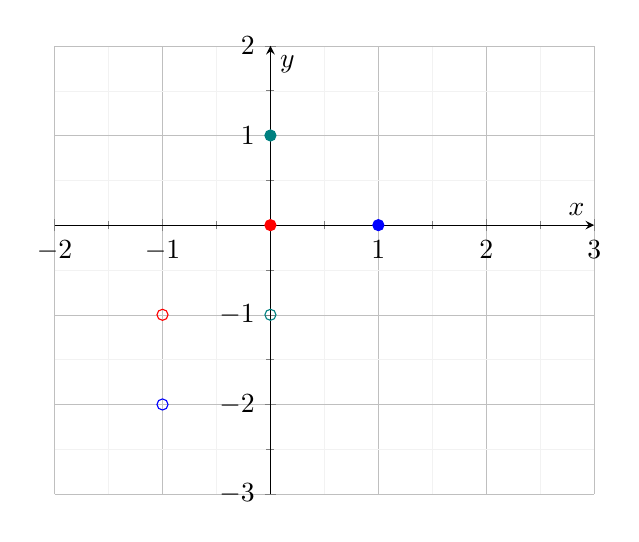
\begin{tikzpicture}
            \begin{axis}[
                axis lines=center,
                xlabel=$x$, ylabel=$y$,
                xmin=-2, xmax=3,
                ymin=-3, ymax=2,
                xtick={-2,...,3},
                ytick={-3,...,2},
                grid=both,
                grid style={line width=.1pt, draw=gray!10},
                major grid style={line width=.2pt,draw=gray!50},
                minor tick num=1,
                clip=false
            ]
                \addplot[only marks,mark=o,red] coordinates {(-1,-1)};
                \addplot[only marks,mark=o,blue] coordinates {(-1,-2)};
                \addplot[only marks,mark=o,teal] coordinates {(0,-1)};

                \addplot[only marks,mark=*,red] coordinates {(0,0)};
                \addplot[only marks,mark=*,blue] coordinates {(1,0)};
                \addplot[only marks,mark=*,teal] coordinates {(0,1)};
            \end{axis}
        \end{tikzpicture}
        \caption{Representación de los puntos dados por el enunciado.}
    \end{figure}

    Definimos en primer lugar el sistema de referencia dado por: $$\cc{R}=\{(-1,-1), (-1,-2), (0,-1)\}.$$
    
    Tenemos que su base asociada es $\cc{B} = \{(0, -1), (1, 0)\}$. Calculemos las imágenes de los vectores de la base mediante $\vec{f}$:
    \begin{gather*}
        \vec{f}(0, -1) = \vec{f(-1, -1)f(-1,-2)} = \vec{(0,0)(1,0)} = (1,0) \\
        \vec{f}(1,0) = \vec{f(-1, -1)f(0, -1)} = \vec{(0,0)(0,1)} = (0,1)
    \end{gather*}

    Tenemos que su matriz asociada es:
    \begin{equation*}
        M(f, \cc{R}, \cc{R}_0) = \left(\begin{array}{c|cc}
            1 & 0 & 0 \\ \hline
            0 & 1 & 0 \\
            0 & 0 & 1
        \end{array}\right)
    \end{equation*}

    En el sistema de referencia usual, tenemos que es:
    \begin{equation*}
        \begin{split}
            M(f, \cc{R}_0) &= M(f, \cc{R}, \cc{R}_0) \cdot M(Id_{\bb{R}^2}, \cc{R}_0, \cc{R}) =\\
            &= M(f, \cc{R}, \cc{R}_0) \cdot M(Id_{\bb{R}^2}, \cc{R}, \cc{R}_0)^{-1} =\\
            &=\left(\begin{array}{c|cc}
                1 & 0 & 0 \\ \hline
                0 & 1 & 0 \\
                0 & 0 & 1
            \end{array}\right)
            \left(\begin{array}{c|cc}
                1 & 0 & 0 \\ \hline
                -1 & 0 & 1 \\
                -1 & -1 & 0
            \end{array}\right)^{-1}
            = \left(\begin{array}{c|cc}
                1 & 0 & 0 \\ \hline
                -1 & 0 & -1 \\
                1 & 1 & 0
            \end{array}\right)
        \end{split}
    \end{equation*}

    Es fácil comprobar que cumple las tres condiciones dadas por el enunciado. Como $\cc{R}_0$ es un sistema de referencia ortonormal, tenemos que para comprobar que $f$ es un movimiento rígido basta con comprobar que $M\left(\vec{f}, \cc{B}_u\right)\in~O(2)$. Tenemos que:
    \begin{equation*}
        M\left(\vec{f}, \cc{B}_u\right)M\left(\vec{f}, \cc{B}_u\right)^t =
        \left(\begin{array}{cc}
                0 & -1 \\
                1 & 0
            \end{array}\right)
            \left(\begin{array}{cc}
                0 & 1 \\
                -1 & 0
            \end{array}\right) = Id_2
    \end{equation*}

    Por tanto, tenemos que es una isometría. Como $\left|\vec{f}\right| = 1$, tenemos que $f$ es una isometría directa. Calculemos los puntos fijos:
    \begin{equation*}
        -\left(\begin{array}{cc}
            -1 & -1 \\
            1 & -1
        \end{array}\right)
        \left(\begin{array}{c}
            x\\y
        \end{array}\right)
        = \left(\begin{array}{c}
            -1 \\1
        \end{array}\right) \Longrightarrow \left\{\begin{array}{l}
            x = -1\\
            y=0
        \end{array}\right.
    \end{equation*}

    Es decir, es una isometría directa con un único punto fijo, por lo que se trata de un giro de ángulo $\theta \neq 0$. Calculemos su ángulo de giro:
    \begin{equation*}
        2\cos\theta = tr\left(M\left(\vec{f}, \cc{B}_u\right)\right) \Longrightarrow \cos\theta  = 0 \Longrightarrow \theta = \frac{\pi}{2}
    \end{equation*}

    Es decir, se trata de giro centrado en el punto $(-1,0)$ y de ángulo $\frac{\pi}{2}$ rad.
\end{ejercicio}

\begin{ejercicio}
    Sea $\cc{R}$ el sistema de referencia de $\bb{R}^2$ con origen en el punto $(1, 1)$ y base asociada $\{(1, 1),(-1, 1)\}$. Consideremos la aplicación afín $f$ tal que, si $(x, y)$ son las coordenadas de un punto genérico $p$ en el sistema de referencia $\cc{R}$, entonces las coordenadas de $f(p)$ en el sistema de referencia usual vienen dadas por
    \begin{equation*}
        f(p)_{\cc{R}_0}=\left(\begin{array}{c}
            -1 \\ 3
        \end{array}\right)+
        \left(\begin{array}{cc}
            1 & 1 \\ 1 & -1
        \end{array}\right)
        \left(\begin{array}{c}
            x \\ y
        \end{array}\right).
    \end{equation*}
    ¿Es $f$ un movimiento rígido? En caso afirmativo, clasifícalo.\\

    Tenemos que $\cc{R}=\{(1,1), \cc{B}\}$, con $\cc{B} = \{(1, 1),(-1, 1)\}$. La matriz asociada de $f$ viene dada por:
    \begin{equation*}
        M(f, \cc{R}, \cc{R}_0) = \left(\begin{array}{c|cc}
            1 & 0 & 0 \\ \hline
            -1 & 1 & 1 \\
            3 & 1 & -1
        \end{array}\right)
    \end{equation*}

    En el sistema de referencia usual, tenemos que es:
    \begin{equation*}
        \begin{split}
            M(f, \cc{R}_0) &= M(f, \cc{R}, \cc{R}_0) \cdot M(Id_{\bb{R}^2}, \cc{R}_0, \cc{R}) =\\
            &= M(f, \cc{R}, \cc{R}_0) \cdot M(Id_{\bb{R}^2}, \cc{R}, \cc{R}_0)^{-1} =\\
            &=\left(\begin{array}{c|cc}
                1 & 0 & 0 \\ \hline
                -1 & 1 & 1 \\
                3 & 1 & -1
            \end{array}\right)
            \left(\begin{array}{c|cc}
                1 & 0 & 0 \\ \hline
                1 & 1 & -1 \\
                1 & 1 & 1
            \end{array}\right)^{-1}
            = \left(\begin{array}{c|cc}
                1 & 0 & 0 \\ \hline
                -2 & 0 & 1 \\
                2 & 1 & 0
            \end{array}\right)
        \end{split}
    \end{equation*}

    Claramente, $\vec{f}$ es una isometría; y como $\left|\vec{f}\right| = -1$, tenemos que es una isometría inversa. Calculemos sus puntos fijos:
    \begin{equation*}
        -\left(\begin{array}{cc}
            -1 & 1 \\
            1 & -1
        \end{array}\right)
        \left(\begin{array}{c}
            x\\y
        \end{array}\right) = 
        \left(\begin{array}{c}
            -2\\2
        \end{array}\right)
    \end{equation*}

    Por tanto, tenemos que hay una recta de puntos fijos: $L\equiv x-y=-2$. Es decir, $L = (-1,1) + \cc{L}\{(1,1)\}$. Como $f$ es una isometría inversa, tenemos que $f$ es una reflexión axial sobre la recta $L$.
\end{ejercicio}

\begin{ejercicio}
    Sean $f_1, f_2 : \bb{R}^3\to \bb{R}^3$ las isometrías dadas respectivamente por las simetrías respecto de los planos de ecuaciones $x + y = 1$ y $x - z = 2$.
    \begin{enumerate}
        \item Calcula explícitamente $f_1$ y $f_2$ en coordenadas usuales.

        Sea $f_1$ la simetría especular respecto de $\pi_1=(0,1,1) + \cc{L}\{(1,-1,0), (0,0,1)\}$. Tenemos que $\vec{\pi_1}^\perp = \cc{L}\{(1,1,0)\}$; por lo que consideramos el sistema de referencia $\cc{R}=\{(0,1,1), \cc{B}\}$, con $\cc{B}=\{(1,-1,0), (0,0,1), (1,1,0)\}$. Tenemos que:
        \begin{equation*}
            M(f_1,\cc{R}) = \left(
            \begin{array}{c|ccc}
                1 & 0 & 0 & 0 \\ \hline
                0 & 1 & 0 & 0 \\
                0 & 0 & 1 & 0 \\
                0 & 0 & 0 & -1
            \end{array}
            \right)
        \end{equation*}

        En las coordenadas usuales, esta es:
        \begin{equation*}
            \begin{split}
                M(f_1,\cc{R}_0) &= M(Id_{\bb{R}^3},\cc{R}, \cc{R}_0) M(f_1,\cc{R}) M(Id_{\bb{R}^3},\cc{R}_0, \cc{R}) =\\
                &= 
                \left(
                \begin{array}{c|ccc}
                    1 & 0 & 0 & 0 \\ \hline
                    0 & 1 & 0 & 1 \\
                    1 & -1 & 0 & 1 \\
                    1 & 0 & 1 & 0
                \end{array}
                \right)
                \left(
                \begin{array}{c|ccc}
                    1 & 0 & 0 & 0 \\ \hline
                    0 & 1 & 0 & 0 \\
                    0 & 0 & 1 & 0 \\
                    0 & 0 & 0 & -1
                \end{array}
                \right)
                \left(
                \begin{array}{c|ccc}
                    1 & 0 & 0 & 0 \\ \hline
                    0 & 1 & 0 & 1 \\
                    1 & -1 & 0 & 1 \\
                    1 & 0 & 1 & 0
                \end{array}
                \right)^{-1}
                =\\
                &=  \left(
                \begin{array}{c|ccc}
                    1 & 0 & 0 & 0 \\ \hline
                    1 & 0 & -1 & 0 \\
                    1 & -1 & 0 & 0 \\
                    0 & 0 & 0 & 1
                \end{array}
                \right)
            \end{split} 
        \end{equation*}



        Sea $f_2$ la simetría especular respecto de $\pi_2=(1,0,-1) + \cc{L}\{(1,0,1), (0,1,0)\}$. Tenemos que $\vec{\pi_2}^\perp = \cc{L}\{(1,0,-1)\}$; por lo que consideramos el sistema de referencia $\cc{R}'=\{(1,0,-1), \cc{B}'\}$, con $\cc{B}'=\{(1,0,1), (0,1,0), (1,0,-1)\}$. Tenemos que:
        \begin{equation*}
            M(f_2,\cc{R}') = \left(
            \begin{array}{c|ccc}
                1 & 0 & 0 & 0 \\ \hline
                0 & 1 & 0 & 0 \\
                0 & 0 & 1 & 0 \\
                0 & 0 & 0 & -1
            \end{array}
            \right)
        \end{equation*}

        En las coordenadas usuales, esta es:
        \begin{equation*}
            \begin{split}
                M(f_2,\cc{R}_0) &= M(Id_{\bb{R}^3},\cc{R}', \cc{R}_0) M(f_2,\cc{R}') M(Id_{\bb{R}^3},\cc{R}_0, \cc{R}') =\\
                &= 
                \left(
                \begin{array}{c|ccc}
                    1 & 0 & 0 & 0 \\ \hline
                    1 & 1 & 0 & 1 \\
                    0 & 0 & 1 & 0 \\
                    -1 & 1 & 0 & -1
                \end{array}
                \right)
                \left(
                \begin{array}{c|ccc}
                    1 & 0 & 0 & 0 \\ \hline
                    0 & 1 & 0 & 0 \\
                    0 & 0 & 1 & 0 \\
                    0 & 0 & 0 & -1
                \end{array}
                \right)
                \left(
                \begin{array}{c|ccc}
                    1 & 0 & 0 & 0 \\ \hline
                    1 & 1 & 0 & 1 \\
                    0 & 0 & 1 & 0 \\
                    -1 & 1 & 0 & -1
                \end{array}
                \right)^{-1}
                =\\
                &=  \left(
                \begin{array}{c|ccc}
                    1 & 0 & 0 & 0 \\ \hline
                    2 & 0 & 0 & 1 \\
                    0 & 0 & 1 & 0 \\
                    -2 & 1 & 0 & 0
                \end{array}
                \right)
            \end{split} 
        \end{equation*}
        
        \item Clasifica el movimiento rígido $g = f_1 \circ f_2$.

        Tenemos que $|g| = |f_1|\cdot |f_2| = 1$, por lo que se trata de una isometría directa en el espacio. Además, tenemos que la recta dada por la intersección de ambos planos es una recta de puntos fijos. Es decir, la recta $L$ dada por:
        \begin{equation*}
            L = \left\{(x,y,z)\in \bb{R}^3 \left|\begin{array}{l}
                x+y=1\\
                x-z=2
            \end{array}\right.\right\} = (0, 1, -2) + \cc{L}\{(1,-1,1)\}
        \end{equation*}
        es una recta de puntos fijos. Como $\vec{f}\neq Id_{\bb{R}^3}$, tenemos que no hay más puntos fijos, por lo que se trata de un giro sobre el eje $L$. Para obtener el ángulo de giro, obtenemos $M(\vec{g},\cc{B}_u)$:
        \begin{equation*}
            \begin{split}
                M(\vec{g},\cc{B}_u) &= M(\vec{f_1\circ f_2},\cc{B}_u) = M(\vec{f_1}\circ \vec{f_2},\cc{B}_u) = M(\vec{f_1},\cc{B}_u)\cdot M(\vec{f_2},\cc{B}_u) =\\
                &= \left(
                \begin{array}{ccc}
                    0 & -1 & 0 \\
                    -1 & 0 & 0 \\
                    0 & 0 & 1
                \end{array}
                \right)
                \left(
                \begin{array}{ccc}
                    0 & 0 & 1 \\
                    0 & 1 & 0 \\
                    1 & 0 & 0
                \end{array}
                \right)
                = \left(
                \begin{array}{ccc}
                    0 & -1 & 0 \\
                    0 & 0 & -1 \\
                    1 & 0 & 0
                \end{array}
                \right)
            \end{split}
        \end{equation*}

        Por tanto, si $\theta$ es el ángulo de giro, tenemos que:
        \begin{equation*}
             1+2\cos\theta = tr(M(\vec{g}, \cc{B}_u)) = 0\Longrightarrow \cos\theta = -\frac{1}{2} \Longrightarrow \theta = \frac{2\pi}{3}
        \end{equation*}
    \end{enumerate}
\end{ejercicio}

\begin{ejercicio}
    Calcula en coordenadas usuales la isometría de $\bb{R}^3$ dada por el movimiento helicoidal alrededor de la recta $R = (1, 2, 1) + \cc{L}\{(1, 0, -1)\}$ con giro de ángulo $\theta = \frac{\pi}{2}$ y vector de traslación $v = (-2, 0, 2)$.\\

    Sea $\vec{R}^\perp = \cc{L}\{(0,1,0), (1,0,1)\}$. Consideramos entonces el sistema de referencia dado por
    $\cc{R}=\{(1,2,1), \cc{B}\}$, con $\cc{B}=\left\{\frac{1}{\sqrt{2}}(1,0,-1), (0,1,0), \frac{1}{\sqrt{2}}(1,0,1)\right\}$. Calculemos las coordenadas de $v$ en $\cc{B}$:
    \begin{equation*}
        v = (-2,0,2) = \alpha\cdot \frac{1}{\sqrt{2}}(1,0,-1) +\beta(0,1,0) + \gamma\cdot \frac{1}{\sqrt{2}}(1,0,1)
    \end{equation*}

    Entonces, $\alpha=-2\sqrt{2}$, $\beta=0$, $\gamma=0$, por lo que $v=(-2\sqrt{2},0,0)_{\cc{B}}$. Entonces, tenemos que:
    \begin{equation*}
        M(f, \cc{R}) = \left(
        \begin{array}{c|ccc}
            1 & 0 & 0 & 0 \\ \hline
            -2\sqrt{2} & 1 & 0 & 0 \\
            0 & 0 & \cos\theta & -\sen\theta \\
            0 & 0 & \sen\theta & \cos\theta
        \end{array}
        \right)
        = \left(
        \begin{array}{c|ccc}
            1 & 0 & 0 & 0 \\ \hline
            -2\sqrt{2} & 1 & 0 & 0 \\
            0 & 0 & 0 & -1 \\
            0 & 0 & 1 & 0
        \end{array}
        \right)
    \end{equation*}

    Para calcular las coordenadas usuales, tenemos que:
    \begin{equation*}
        \begin{split}
            M(f, \cc{R}_0) &= M(Id_{\bb{R}^3}, \cc{R}, \cc{R}_0) \cdot M(f, \cc{R}) \cdot M(Id_{\bb{R}^3}, \cc{R}_0, \cc{R}) =\\
            &= M(Id_{\bb{R}^3}, \cc{R}, \cc{R}_0) \cdot M(f, \cc{R}) \cdot M(Id_{\bb{R}^3}, \cc{R}, \cc{R}_0)^{-1} =\\
            &=\frac{1}{\sqrt{2}}\left(
            \begin{array}{c|ccc}
                \sqrt{2} & 0 & 0 & 0 \\ \hline
                \sqrt{2} & 1 & 0 & 1 \\
                2\sqrt{2} & 0 & \sqrt{2} & 0 \\
                \sqrt{2} & -1 & 0 & 1
            \end{array}
            \right)
            \left(
            \begin{array}{c|ccc}
                1 & 0 & 0 & 0 \\ \hline
                -2\sqrt{2} & 1 & 0 & 0 \\
                0 & 0 & 0 & -1 \\
                0 & 0 & 1 & 0
            \end{array}
            \right)
            \cdot \\& \hspace{4cm} \cdot \sqrt{2}
            \left(
            \begin{array}{c|ccc}
                \sqrt{2} & 0 & 0 & 0 \\ \hline
                \sqrt{2} & 1 & 0 & 1 \\
                2\sqrt{2} & 0 & \sqrt{2} & 0 \\
                \sqrt{2} & -1 & 0 & 1
            \end{array}
            \right)^{-1}
            =\\
            &= \frac{1}{2} \left(
            \begin{array}{c|ccc}
                2 & 0 & 0 & 0 \\ \hline
                -2\sqrt{2}-2 & 1 & \sqrt{2} & -1 \\
                2\sqrt{2}+4 & -\sqrt{2} & 0 & -\sqrt{2}\\
                -2\sqrt{2}+6 & -1 & \sqrt{2} & 1
            \end{array}
            \right)
        \end{split}
    \end{equation*}
\end{ejercicio}

\begin{ejercicio}
    Clasifica el siguiente movimiento rígido de $\bb{R}^3$:
    \begin{equation*}
        f(x, y, z) = \frac{1}{3}(2x + 2y + z + 2, x - 2y + 2z - 2, 2x - y - 2z - 4)
    \end{equation*}
    y calcula sus elementos notables (o geométricos).

    Tenemos que su matriz asociada en el sistema de referencia usual es:
    \begin{equation*}
        M(f, \cc{R}_0) = \frac{1}{3}\left(
        \begin{array}{c|ccc}
            3 & 0 & 0 & 0 \\ \hline
            2 & 2 & 2 & 1 \\
            -2 & 1 & -2 & 2 \\
            -4 & 2 & -1 & -2
        \end{array}
        \right)
    \end{equation*}

    Tenemos que $|f| = 1$, por lo que se trata de una isometría directa. Calculemos sus puntos fijos:
    \begin{equation*}
        \left(
        \begin{array}{ccc}
            -1 & 2 & 1 \\
            1 & -5 & 2 \\
            2 & -1 & -5
        \end{array}
        \right)
        \left(
        \begin{array}{c}
            x \\ y \\ z
        \end{array}
        \right)
        = \left(
        \begin{array}{c}
            -2 \\ 2 \\ 4
        \end{array}
        \right)
        \Longrightarrow \left\{\begin{array}{l}
            x = 2+3\lm\\
            y = \lm\\
            z = \lm
        \end{array}\right.
    \end{equation*}

    Por tanto, tenemos que $f$ es una isometría directa en el espacio con una recta de puntos fijos, por lo que se trata de un giro. Tenemos que el eje de giro es la recta $L$ dada por:
    \begin{equation*}
        L = (2,0,0) + \cc{L}\left\{(3,1,1)\right\}
    \end{equation*}

    Calculemos ahora el ángulo de giro no orientado $\theta \in [0, \pi]$. Como la traza de la matriz queda invariantes por semejanza, tenemos que:
    \begin{equation*}
        1+2\cos\theta = tr\left(M\left(\vec{f}, \cc{B}_u\right)\right) = \frac{1}{3}(2 -2 -2) \Longrightarrow \cos\theta = -\frac{5}{6} \Longrightarrow \theta \approx 2.55 \text{ rad}
    \end{equation*}
\end{ejercicio}

\begin{ejercicio}
    Calcula la simetría con deslizamiento respecto del plano de ecuación $x + y + z = 1$ de $\bb{R}^3$ y con vector de traslación $v = (2, -1, -1)$.

    Tenemos que el plano de simetría es $\pi = (1,0,0) + \cc{L}\left\{(1,-1,0), (1,0,-1)\right\}$. Entonces, $\vec{\pi}^\perp = \cc{L}\left\{(1,1,1)\right\}$.
    Consideramos entonces el sistema de referencia dado por:
    \begin{equation*}
        \cc{R} = \left\{(1,0,0), \cc{B}\right\}, \text{ con } \cc{B} = \left\{(1,-1,0), (1,0,-1), (1,1,1)\right\}
    \end{equation*}

    Calculamos las coordenadas de $v$ en $\cc{B}$:
    \begin{equation*}
        v = (2,-1,-1) = \alpha\cdot (1,-1,0) + \beta\cdot (1,0,-1) + \gamma\cdot (1,1,1)
    \end{equation*}
    Igualando cada componente, tenemos que $\alpha = 1$, $\beta = 1$, $\gamma = 0$. Por tanto, $v = (1,1,0)_{\cc{B}}$. Entonces, tenemos que:
    \begin{equation*}
        M(f, \cc{R}) = \left(
        \begin{array}{c|ccc}
            1 & 0 & 0 & 0 \\ \hline
            1 & 1 & 0 & 0 \\
            1 & 0 & 1 & 0 \\
            0 & 0 & 0 & -1
        \end{array}
        \right)
    \end{equation*}

    Para calcular la matriz en el sistema de referencia usual (aunque no nos lo piden), tenemos que:
    \begin{equation*}
        \begin{split}
            M(f, \cc{R}_0) &= M(Id_{\bb{R}^3}, \cc{R}, \cc{R}_0) \cdot M(f, \cc{R}) \cdot M(Id_{\bb{R}^3}, \cc{R}_0, \cc{R}) =\\
            &= M(Id_{\bb{R}^3}, \cc{R}, \cc{R}_0) \cdot M(f, \cc{R}) \cdot M(Id_{\bb{R}^3}, \cc{R}, \cc{R}_0)^{-1} =\\
            &=\left(
            \begin{array}{c|ccc}
                1 & 0 & 0 & 0 \\ \hline
                1 & 1 & 1 & 1 \\
                0 & -1 & 0 & 1 \\
                0 & 0 & -1 & 1
            \end{array}
            \right)
            \left(
            \begin{array}{c|ccc}
                1 & 0 & 0 & 0 \\ \hline
                1 & 1 & 0 & 0 \\
                1 & 0 & 1 & 0 \\
                0 & 0 & 0 & -1
            \end{array}
            \right)\left(
            \begin{array}{c|ccc}
                1 & 0 & 0 & 0 \\ \hline
                1 & 1 & 1 & 1 \\
                0 & -1 & 0 & 1 \\
                0 & 0 & -1 & 1
            \end{array}
            \right)^{-1}
            =\\
            &= \frac{1}{3} \left(
            \begin{array}{c|ccc}
                3 & 0 & 0 & 0 \\ \hline
                8 & 1 & -2 & -2 \\
                -1 & -2 & 1 & -2 \\
                -1 & -2 & -2 & 1
            \end{array}
            \right)
        \end{split}
    \end{equation*}
\end{ejercicio}

\begin{ejercicio}
    Clasifica el movimiento rígido de $\bb{R}^3$ dado por
    \begin{equation*}
        f(x,y,z) = \left(
        \frac{2x+2y+z+3}{3}, \frac{-2x+y+2z}{3}, \frac{-x+2y-2z-3}{3}
        \right)
    \end{equation*}

    Tenemos que su matriz asociada en el sistema de referencia usual es:
    \begin{equation*}
        M(f, \cc{R}_0) = \frac{1}{3}\left(
        \begin{array}{c|ccc}
            3 & 0 & 0 & 0 \\ \hline
            3 & 2 & 2 & 1 \\
            0 & -2 & 1 & 2 \\
            -3 & -1 & 2 & -2
        \end{array}
        \right)
    \end{equation*}

    Tenemos que $|f| = -1$, por lo que se trata de una isometría inversa. Calculemos sus puntos fijos:
    \begin{equation*}
        \left(
        \begin{array}{ccc}
            -1 & 2 & 1 \\
            -2 & -2 & 2 \\
            -1 & 2 & -5
        \end{array}
        \right)
        \left(
        \begin{array}{c}
            x \\ y \\ z
        \end{array}
        \right)
        = \left(
        \begin{array}{c}
            -3 \\ 0 \\ 3
        \end{array}
        \right)
        \Longrightarrow \left\{\begin{array}{l}
            x = 0\\
            y = -1\\
            z = -1
        \end{array}\right.
    \end{equation*}

    Por tanto, tenemos que $f$ es una isometría inversa en el espacio con un único punto fijo, por lo que se trata de un giro con simetría.
    Calculemos el eje de giro:
    \begin{align*}
        \vec{L} &= V_{-1} = \left\{(x,y,z)\in \bb{R}^3 \left|
            \left(M\left(\vec{f},\cc{B}_u\right) +Id\right)(x,y,z)^t = 0
        \right.\right\} =\\
        &= \left\{(x,y,z)\in \bb{R}^3 \left|
            \left(
            \begin{array}{ccc}
                5 & 2 & 1 \\
                -2 & 4 & 2 \\
                -1 & 2 & 1
            \end{array}
            \right)
            \left(
            \begin{array}{c}
                x \\ y \\ z
            \end{array}
            \right)
            = 0
        \right.\right\} =\\
        &= \left\{(x,y,z)\in \bb{R}^3 \left|
            \left(
            \begin{array}{ccc}
                5 & 2 & 1 \\
                12 & 0 & 0 \\
            \end{array}
            \right)
            \left(
            \begin{array}{c}
                x \\ y \\ z
            \end{array}
            \right)
            = 0
        \right.\right\} =\\
        &= \cc{L}\left(0, 1, -2\right)
    \end{align*}

    Por tanto, tenemos que el eje es la recta $L$ dada por:
    \begin{equation*}
        L = (0,-1,-1) + \cc{L}\left(0, 1, -2\right)
    \end{equation*}

    Calculemos ahora el ángulo de giro no orientado $\theta \in [0, \pi]$. Como la traza de la matriz queda invariantes por semejanza, tenemos que:
    \begin{equation*}
        -1+2\cos\theta = tr\left(M\left(\vec{f}, \cc{B}_u\right)\right) = \frac{1}{3}(2+1-2) \Longrightarrow \cos\theta = \frac{2}{3} \Longrightarrow \theta \approx 0.84 \text{ rad}
    \end{equation*}
\end{ejercicio}

\begin{ejercicio}
    Calcula la isometría de $\bb{R}^3$ dada por la composición de un giro de ángulo $\frac{\pi}{2}$ respecto del eje $R \equiv (1, 2, 0) + \cc{L}(\{(0, 1, 0)\})$ y la simetría respecto del plano $y = -1$.

    \begin{figure}[H]
        \centering
        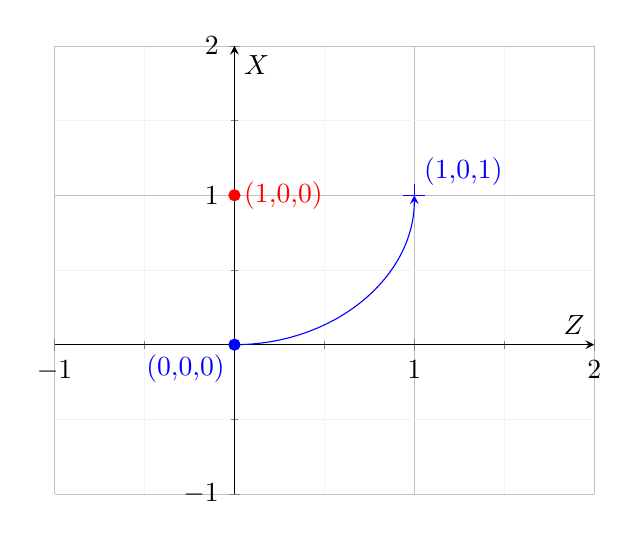
\begin{tikzpicture}
            \shorthandoff{"}
            \begin{axis}[
                axis lines=center,
                xlabel=$Z$, ylabel=$X$,
                xmin=-1, xmax=2,
                ymin=-1, ymax=2,
                xtick={-1,...,2},
                ytick={-1,...,2},
                grid=both,
                grid style={line width=.1pt, draw=gray!10},
                major grid style={line width=.2pt,draw=gray!50},
                minor tick num=1,
                clip=false
            ]
                \addplot[only marks,red, nodes near coords={(1,0,0)}, every node near coord/.append style={red, anchor=west}] coordinates {(0,1)};
                \addplot[only marks,red] coordinates {(0,1)};
                
                \addplot[only marks,blue, nodes near coords={(0,0,0)}, every node near coord/.append style={blue, anchor=north east}] coordinates {(0,0)};
                \addplot[only marks,blue] coordinates {(0,0)};

                \addplot[only marks,blue, nodes near coords={(1,0,1)}, every node near coord/.append style={blue, anchor=south west}] coordinates {(1,1)};
                \addplot[only marks,blue, mark=+, mark options={scale=2}] coordinates {(1,1)};
                \draw[blue, stealth-] (axis cs:1,1) arc[start angle=0, end angle=-90, radius=1];
            \end{axis}
            \shorthandon{"}
        \end{tikzpicture}
        \caption{Giro de ángulo $\frac{\pi}{4}$ en el plano $R^\perp_{(1,0,0)}$, es decir, el plano $y=0$ ($XZ$).}
    \end{figure}

    Calculamos en primer lugar la matriz asociada al giro de ángulo $\frac{\pi}{2}$ respecto del eje $R$. Como $\vec{R}^\perp = \cc{L}\{e_1, e_3\}$, tenemos que:
    \begin{equation*}
        G_{\theta, \vec{L}}(e_1) = -e_3, \quad G_{\theta, \vec{L}}(e_2) = e_2, \quad G_{\theta, \vec{L}}(e_3) = e_1 \qquad G_{\theta, L}(0,0,0) = (1,0,1)
    \end{equation*}

    Por tanto, la matriz asociada en el sistema de referencia usual es:
    \begin{equation*}
        M(G_{\theta, {L}}, \cc{R}_0) = \left(
        \begin{array}{c|ccc}
            1 & 0 & 0 & 0 \\ \hline
            1 & 0 & 0 & 1 \\
            0 & 0 & 1 & 0 \\
            1 & -1 & 0 & 0
        \end{array}
        \right)
    \end{equation*}

    Calculamos ahora la matriz asociada a la simetría respecto del plano $\pi\equiv y=-1$. Tenemos que:
    \begin{equation*}
        \sigma_{\vec{\pi}}(e_1) = e_1, \quad \sigma_{\vec{\pi}}(e_2) = -e_2, \quad \sigma_{\vec{\pi}}(e_3) = e_3 \qquad \sigma_{{\pi}}(0,0,0) = (0,-2,0)
    \end{equation*}

    Por tanto, la matriz asociada en el sistema de referencia usual es:
    \begin{equation*}
        M(\sigma_{{\pi}}, \cc{R}_0) = \left(
        \begin{array}{c|ccc}
            1 & 0 & 0 & 0 \\ \hline
            0 & 1 & 0 & 0 \\
            -2 & 0 & -1 & 0 \\
            0 & 0 & 0 & 1
        \end{array}
        \right)
    \end{equation*}

    Por tanto, la matriz asociada a la composición de ambas isometrías es:
    \begin{align*}
        M(f, \cc{R}_0) &= M(\sigma_{{\pi}}, \cc{R}_0) \cdot M(G_{\theta, {L}}, \cc{R}_0) =\\
        &= \left(
        \begin{array}{c|ccc}
            1 & 0 & 0 & 0 \\ \hline
            0 & 1 & 0 & 0 \\
            -2 & 0 & -1 & 0 \\
            0 & 0 & 0 & 1
        \end{array}
        \right)
        \left(
        \begin{array}{c|ccc}
            1 & 0 & 0 &  \\ \hline
            1 & 0 & 0 & 1 \\
            0 & 0 & 1 & 0 \\
            1 & -1 & 0 & 0
        \end{array}
        \right)
        =\\
        &= \left(
        \begin{array}{c|ccc}
            1 & 0 & 0 & 0 \\ \hline
            1 & 0 & 0 & 1 \\
            -2 & 0 & -1 & 0 \\
            1 & -1 & 0 & 0
        \end{array}
        \right)
    \end{align*}
\end{ejercicio}

\begin{ejercicio}
    Para cada $\alpha \in \bb{R}$ se considera el movimiento rígido de $\bb{R}^3$ dado por:
    \begin{equation*}
        f_\alpha(x,y,z)=\frac{1}{3}(-x + 2y + 2z + 2, 2x + 2y - z - 1, 2x - y + 2z - \alpha).
    \end{equation*}
    Clasificar, según los valores de $\alpha$, qué tipo de movimiento es $f_\alpha$, calculando en cada caso el conjunto de puntos fijos.

    Tenemos que su matriz asociada en el sistema de referencia usual es:
    \begin{equation*}
        M(f_\alpha, \cc{R}_0) = \frac{1}{3}\left(
        \begin{array}{c|ccc}
            3 & 0 & 0 & 0 \\ \hline
            2 & -1 & 2 & 2 \\
            -1 & 2 & 2 & -1 \\
            -\alpha & 2 & -1 & 2
        \end{array}
        \right)
    \end{equation*}

    Tenemos que $|f_\alpha| = -1$, por lo que se trata de una isometría inversa. Calculemos sus puntos fijos:
    \begin{equation*}
        \left(
        \begin{array}{ccc}
            -4 & 2 & 2 \\
            2 & -1 & -1 \\
            2 & -1 & -1
        \end{array}
        \right)
        \left(
        \begin{array}{c}
            x \\ y \\ z
        \end{array}
        \right)
        = \left(
        \begin{array}{c}
            -2 \\ 1 \\ \alpha
        \end{array}
        \right)
    \end{equation*}

    Realizamos una distinción de casos en función del parámetro $\alpha$:
    \begin{itemize}
        \item Si $\alpha \neq 1$:
        
        Tenemos que el sistema es SI, por lo que $\cc{P}_f=\emptyset$. Se trata de una simetría especular con deslizamiento.

        \item Si $\alpha = 1$:
        
        Tenemos que el sistema es SCI, y hay un plano de puntos fijos. Por tanto, se trata de una simetría especular respecto del plano $\pi$ dado por:
        \begin{equation*}
            \pi \equiv 2x-y-z=1 \equiv (1,1,0) + \cc{L}\left\{(1,1,1)\right\}
        \end{equation*}
    \end{itemize}
\end{ejercicio}

\begin{ejercicio}
    Sea $\cc{R}$ es el sistema de referencia con origen en el punto $(1, 0, 1)$ y base asociada $\{(1, 0, 0),(1, 1, 0),(1, 1, 1)\}$. Determina si la siguiente aplicación afín $f : \bb{R}^3\to \bb{R}^3$, que en coordenadas respecto del sistema de referencia afín $\cc{R}$ está dada por
    \begin{equation*}
        f\left(\begin{array}{c}
            x \\ y \\ z
        \end{array}\right) = \frac{1}{5}
        \left[
        \left(\begin{array}{c}
            -9 \\ 16 \\ -7
        \end{array}\right) +
        \left(\begin{array}{ccc}
            5 & 2 & -2 \\
            0 & 7 & 8 \\
            0 & -4 & -1
        \end{array}\right)
        \left(\begin{array}{c}
            x \\ y \\ z
        \end{array}\right)
        \right]
    \end{equation*}
    es un movimiento rígido y, en caso afirmativo, clasifícalo.\\

    Tenemos que:
    \begin{equation*}
        M(f, \cc{R}) = \frac{1}{5}\left(
        \begin{array}{c|ccc}
            5 & 0 & 0 & 0 \\ \hline
            -9 & 5 & 2 & -2 \\
            16 & 0 & 7 & 8 \\
            -7 & 0 & -4 & -1
        \end{array}
        \right)
    \end{equation*}

    Tenemos que $\cc{R}$ no es ortonormal, por lo que calcularemos su matriz en el sistema de referencia usual para determinar si es un movimiento rígido.
    \begin{align*}
        M(f, \cc{R}_0) &= M(Id_{\bb{R}^3}, \cc{R}, \cc{R}_0) \cdot M(f, \cc{R}) \cdot M(Id_{\bb{R}^3}, \cc{R}_0, \cc{R}) =\\
        &= M(Id_{\bb{R}^3}, \cc{R}, \cc{R}_0) \cdot M(f, \cc{R}) \cdot M(Id_{\bb{R}^3}, \cc{R}, \cc{R}_0)^{-1} =\\
        &=\left(
        \begin{array}{c|ccc}
            1 & 0 & 0 & 0 \\ \hline
            1 & 1 & 1 & 1 \\
            0 & 0 & 1 & 1 \\
            1 & 0 & 0 & 1
        \end{array}
        \right) \cdot \frac{1}{5}\cdot 
        \left(
        \begin{array}{c|ccc}
            5 & 0 & 0 & 0 \\ \hline
            -9 & 5 & 2 & -2 \\
            16 & 0 & 7 & 8 \\
            -7 & 0 & -4 & -1
        \end{array}
        \right)\left(
        \begin{array}{c|ccc}
            1 & 0 & 0 & 0 \\ \hline
            1 & 1 & 1 & 1 \\
            0 & 0 & 1 & 1 \\
            1 & 0 & 0 & 1
        \end{array}
        \right)^{-1}
        =\\
        &= \frac{1}{5}\left(
        \begin{array}{c|ccc}
            5 & 0 & 0 & 0 \\ \hline
            0 & 5 & 0 & 0 \\
            5 & 0 & 3 & 4 \\
            -5 & 0 & -4 & 3
        \end{array}
        \right)
    \end{align*}

    Tenemos que:
    \begin{equation*}
        |f| = \frac{1}{5^4} \cdot 5^2 \cdot (9 + 16) = 1
    \end{equation*}

    Por tanto, se trata de una isometría directa. Calculemos sus puntos fijos:
    \begin{equation*}
        \left(
        \begin{array}{ccc}
            0 & 0 & 0 \\
            0 & -2 & 4 \\
            0 & -4 & -2
        \end{array}
        \right)
        \left(
        \begin{array}{c}
            x \\ y \\ z
        \end{array}
        \right)
        = \left(
        \begin{array}{c}
            0 \\ -5 \\ 5
        \end{array}
        \right) \Longrightarrow \left\{\begin{array}{l}
            x = \lm \in \bb{R}\\
            y = -\nicefrac{1}{2}\\
            z = -\nicefrac{3}{2}
        \end{array}\right. \Longrightarrow \cc{P}_f = \left(0, -\frac{1}{2}, -\frac{3}{2}\right) + \cc{L}\left(1,0,0\right)
    \end{equation*}

    Por tanto, tenemos que hay una recta de puntos fijos, por lo que se trata de un giro respecto de dicha recta. Calculemos el ángulo de giro no orientado $\theta \in [0, \pi]$.
    \begin{equation*}
        1+2\cos\theta = tr\left(M\left(\vec{f}, \cc{B}_u\right)\right) = \frac{1}{5}(5+3+3) \Longrightarrow \cos\theta = \frac{3}{5} \Longrightarrow \theta = \arccos\left(\frac{3}{5}\right) \approx 0.927 \text{ rad}
    \end{equation*}
\end{ejercicio}

\begin{ejercicio}
    Decide de forma razonada qué tipo de movimiento rígido es:
    \begin{enumerate}
        \item La composición de dos simetrías ortogonales en el plano euclídeo $\bb{R}^2$.
        
        Sea $f$ dicha composición. Como $|f|=1$, tenemos que se trata de una isometría directa. Distinguimos en función de la posición relativa de ambas rectas:
        \begin{itemize}
            \item Si $R_1=R_2$ (son coincidentes), entonces veamos que $f=Id_{\bb{R}^2}$.
            
            Tenemos que $f=\sigma_{R_1} \circ \sigma_{R_2}=\sigma_{R_1} \circ \sigma_{R_1} \AstIg Id_{\bb{R}^2}$,
            donde en $(\ast)$ he aplicado la propiedad de involución de las simetrías.

            \item Si $R_1 \| R_2$, $R_1 \neq R_2$ (son paralelas), entonces veamos que $f$ es una traslación según un vector no nulo. Tenemos que:
            \begin{equation*}
                \vec{f} = \vec{\sigma_{R_1}} \circ \vec{\sigma_{R_2}} = \sigma_{\vec{R_1}} \circ \sigma_{\vec{R_1}} \AstIg Id_{\bb{R}^2}
            \end{equation*}
            donde en $(\ast)$ he aplicado la propiedad de involución de las simetrías vectoriales. Veamos ahora que el vector no es nulo.
            Sea $p\in R_2$, entonces $\sigma_{R_2}(p)=p$. Por tanto, $f(p)=\sigma_{R_1}(p)$. Como $R_1 \neq R_2$, tenemos que $\sigma_{R_1}(p) \neq p$, por lo que:
            \begin{equation*}
                \vec{p~f(p)} = \vec{p~\sigma_{R_1}(p)} \neq \vec{0}
            \end{equation*}
            Además, sabemos que $\vec{p~f(p)} = \vec{p~\sigma_{R_1}(p)} \in \vec{R_1}^\perp$.
            Por tanto, como su lineal asociada es la identidad y su vector de traslación es no nulo, se trata de una traslación sin puntos fijos.

            \item Si $R_1\cap R_2 \neq \emptyset$, $R_1 \cancel{\|} R_2$ (son secantes), entonces veamos que $f$ es un giro de ángulo $\theta \in ]0, \pi]$.
            
            En primer lugar, veamos que $f$ tiene tan solo un punto fijo. Veamos en primer lugar la existencia de dicho punto.
            Sea $R_1\cap R_2 = \{p\}$. Entonces, $\sigma_{R_1}(p)=p$ y $\sigma_{R_2}(p)=p$. Por tanto, $f(p)=\sigma_{R_1} \circ \sigma_{R_2}(p)=p$.
            
            Veamos ahora la unicidad. Como $f$ es un movimiento directo en el plano, basta con que haya algún punto que no sea fijo para que no haya más.
            Sea $q\in R_2,~q\neq p$. Entonces, $\sigma_{R_2}(q)=q$. Por tanto, $f(q)=\sigma_{R_1} \circ \sigma_{R_2}(q) = \sigma_{R_1}(q)$. Como $q\notin R_1$, entonces $f(q)\neq q$.

            Por tanto, sabemos que se trata de un giro de centro $p$ de ángulo no orientado $\theta \in ]0, \pi]$.
        \end{itemize}


        \item La composición de dos simetrías ortogonales con deslizamiento en el plano euclídeo $\bb{R}^2$.
        
        Sea $f_1 = t_{v_1} \circ \sigma_{R_1}$ y $f_2 = t_{v_2} \circ \sigma_{R_2}$, con $v_1\in \vec{R_1}\setminus \{0\}$ y $v_2\in \vec{R_2}\setminus \{0\}$.
        Por tanto, tenemos que:
        \begin{equation*}
            f = f_1 \circ f_2 = t_{v_1} \circ \sigma_{R_1} \circ t_{v_2} \circ \sigma_{R_2} = t_{v_1} \circ t_{v_2} \circ \sigma_{R_1} \circ \sigma_{R_2}
            = t_{v_1+v_2} \circ \sigma_{R_1} \circ \sigma_{R_2}
        \end{equation*}

        Por tanto, haremos uso del apartado anterior para clasificar la composición de las simetrías ortogonales $\sigma_{R_1} \circ \sigma_{R_2}$.
        \begin{itemize}
            \item Si $v_1+v_2 = 0$, entonces la clasificación es la misma que en el apartado anterior.
            \item Si $v_1+v_2 \neq 0$, entonces tenemos que:
            \begin{itemize}
                \item Si $R_1=R_2$ (son coincidentes), entonces sabemos que $\sigma_{R_1} \circ \sigma_{R_2}= Id_{\bb{R}^2}$,
                por lo que $f=t_{v_1+v_2}$, que se trata de una traslación sin puntos fijos.
                
                \item Si $R_1 \| R_2$, $R_1 \neq R_2$ (son paralelas),
                entonces sabemos que $\sigma_{R_1} \circ \sigma_{R_2}=t_v$, con $v\in \vec{R_1}^\perp \setminus \{0\}$.
                Como $v\in \vec{R_1}^\perp$ y $v_1+v_2 \in \vec{R_1}$, tenemos que $v\perp v_1+v_2$, por lo que $v_1+v_2+v \neq 0$.
                por lo que $f=t_{v_1+v_2+v}$, que se trata de una traslación sin puntos fijos.
                
                \item Si $R_1\cap R_2 \neq \emptyset$, $R_1 \cancel{\|} R_2$ (son secantes), 
                sabemos que $\sigma_{R_1} \circ \sigma_{R_2}$ es un giro de centro $p$ de ángulo no orientado $\theta \in ]0, \pi]$.

                Por tanto, tenemos que:
                \begin{equation*}
                    \vec{f} = \vec{t_{v_1+v_2}} \circ \vec{G_{\theta, p}} = Id_{\bb{R}^2} \circ G_{\theta} = G_{\theta}
                \end{equation*}

                Como $\theta \neq 0$, tenemos que $f$ es un giro de ángulo no orientado $\theta \in ]0, \pi]$.
            \end{itemize}
        \end{itemize}


        \item La composición de un giro y una simetría en el plano euclídeo $\bb{R}^2$.
        
        En este caso, tenemos que $f = G_{\theta, p} \circ \sigma_{R}$, con $p\in \bb{R}^2$, $\theta \in ]0, \pi]$ y $R\subset \bb{R}^2$.
        Tenemos que $|f| = -1$, por lo que se trata de una isometría inversa.
        Por tanto, se trata de una simetría axial o una simetría axial con deslizamiento. Supongamos que
        es una simetría axial con deslizamiento, $t_v\circ \sigma_{S}$, con $v\in \vec{S}\setminus \{0\}$. Tenemos que:
        \begin{equation*}
            G_{\theta, p} \circ \sigma_{R} = t_v\circ \sigma_{S} \Longrightarrow
            G_{\theta, p} = t_v\circ \sigma_{S} \circ \sigma_{R}
        \end{equation*}

        Distinguimos en funión de la posición relativa de $S$ y $R$:
        \begin{itemize}
            \item Si $S=R$ (son coincidentes), entonces sabemos que $\sigma_{S} \circ \sigma_{R}= Id_{\bb{R}^2}$,
            por lo que $G_{\theta, p}=t_v$, llegando a una contradicción, ya que el giro tiene puntos fijos pero la traslación no.

            \item Si $S \| R$, $S \neq R$ (son paralelas), entonces sabemos que $\sigma_{S} \circ \sigma_{R}=t_w$, con $w\in \vec{S}^\perp \setminus \{0\}$.
            Como $w\in \vec{S}^\perp$ y $v\in \vec{S}$, tenemos que $w\perp v$, por lo que $v+w \neq 0$.
            por lo que $G_{\theta, p}=t_{v+w}$. Esto es una contradicción, ya que el giro tiene puntos fijos pero la traslación no.

            \item Si $S\cap R \neq \emptyset$, $S \cancel{\|} R$ (son secantes),
            sabemos que $\sigma_{S} \circ \sigma_{R}$ es un giro de centro $q$ de ángulo no orientado $\theta' \in ]0, \pi]$.
            Por tanto, tenemos que $G_{\theta, p} = t_v\circ G_{\theta', q}$,
            que también es una contradicción, ya que $p$ no se mantiene fijo en el caso de la derecha.
        \end{itemize}
        
        Por tanto, se trata de una simetría axial.


        \item La composición de un giro y una simetría con deslizamiento en el plano euclídeo~$\bb{R}^2$.
        
        En este caso, tenemos que $f = G_{\theta, p} \circ \sigma_{R} \circ t_v$, con $p\in \bb{R}^2$, $\theta \in ]0, \pi]$, $v\in \vec{R}\setminus \{0\}$ y
        $R\subset \bb{R}^2$. Por el apartado anterior, sabemos que $G_{\theta, p} \circ \sigma_{R}$ es una simetría axial, sea esta $\sigma_{S}$, con $S\subset \bb{R}^2$.

        Por tanto, tenemos que:
        \begin{equation*}
            f=G_{\theta, p} \circ \sigma_{R} \circ t_v = \sigma_{S} \circ t_v \qquad v\in \vec{R}\setminus \{0\}
        \end{equation*}

        Además, sabemos que $|f| = -1$, por lo que se trata de una isometría inversa. Por tanto, se trata de una simetría axial con o sin deslizamiento.

        % // TODO: Composición de un giro y una simetría con deslizamiento en R2$.

        \item La composición de dos simetrías ortogonales en el espacio euclídeo $\bb{R}^3$.
        
        Sean $f_1 = \sigma_{\pi_1}$ y $f_2 = \sigma_{\pi_2}$, con $\pi_1$ y $\pi_2$ dos planos.
        Sea $f = f_1 \circ f_2$, y tenemos que $|f| = 1$, por lo que se trata de una isometría directa.
        Distinguimos en función de la posición relativa de ambos planos:
        \begin{itemize}
            \item Si $\pi_1=\pi_2$ (son coincidentes), entonces veamos que $f=Id_{\bb{R}^3}$.
            
            Tenemos que $f=\sigma_{\pi_1} \circ \sigma_{\pi_2}=\sigma_{\pi_1} \circ \sigma_{\pi_1} \AstIg Id_{\bb{R}^3}$,
            donde en $(\ast)$ he aplicado la propiedad de involución de las simetrías.

            \item Si $\pi_1 \| \pi_2$, $\pi_1 \neq \pi_2$ (son paralelos), entonces veamos que $f$ es una traslación según un vector no nulo. Tenemos que:
            \begin{equation*}
                \vec{f} = \vec{\sigma_{\pi_1}} \circ \vec{\sigma_{\pi_2}} = \sigma_{\vec{\pi_1}} \circ \sigma_{\vec{\pi_1}} \AstIg Id_{\bb{R}^3}
            \end{equation*}
            donde en $(\ast)$ he aplicado la propiedad de involución de las simetrías vectoriales. Veamos ahora que el vector no es nulo.
            Sea $p\in \pi_2$, entonces $\sigma_{\pi_2}(p)=p$. Por tanto, $f(p)=\sigma_{\pi_1}(p)$. Como $\pi_1 \neq \pi_2$, tenemos que $\sigma_{\pi_1}(p) \neq p$, por lo que:
            \begin{equation*}
                \vec{p~f(p)} = \vec{p~\sigma_{\pi_1}(p)} \neq \vec{0}
            \end{equation*}
            Además, sabemos que $\vec{p~f(p)} = \vec{p~\sigma_{\pi_1}(p)} \in \vec{\pi_1}^\perp$.
            Por tanto, como su lineal asociada es la identidad y su vector de traslación es no nulo, se trata de una traslación sin puntos fijos.

            \item Si $\dim \pi_1 \cap \pi_2 = 0$, veamos que no es posible. Por la fórmula de las dimensiones, como la intersección no es nula, tenemos que:
            \begin{equation*}
                \dim \pi_1 + \dim \pi_2 = \dim (\pi_1 \cap \pi_2) + \dim (\pi_1 \vee \pi_2) \Longrightarrow 4 = 0 + \dim (\pi_1 \vee \pi_2)
            \end{equation*}
            No obstante, esto es una contradicción, ya que $\dim (\pi_1 \vee \pi_2) \leq 3$.

            \item Si $\dim \pi_1 \cap \pi_2 = 1$, entonces hay una recta de puntos fijos.
            Veamos que hay algún punto que no es fijo. Sea $p\in \pi_2$, entonces $\sigma_{\pi_2}(p)=p$. Por tanto, $f(p)=\sigma_{\pi_1}(p)$. Como $\pi_1 \neq \pi_2$, $p\notin \pi_1$, por lo que $\sigma_{\pi_1}(p) \neq p$.
            por tanto, $f\neq Id_{\bb{R}^3}$, y por ser $f$ un movimiento directo tenemos que $f$ es un giro de eje $\pi_1 \cap \pi_2$ y ángulo no orientado $\theta \in ]0, \pi]$.
        \end{itemize}

        \item La composición de un giro y una simetría en el espacio euclídeo $\bb{R}^3$.
        
        Sea $f = G_{\theta, L} \circ \sigma_{\pi}$, con $L$ una recta, $\theta \in ]0, \pi]$ y $\pi$ un plano.
        Tenemos que $|f| = -1$, por lo que se trata de una isometría inversa. Según la posición relativa de $L$ respecto de $\pi$, tenemos:
        \begin{itemize}
            \item Si $L\subset \pi$, entonces veamos que se trata de una reflexión especular.
            
            Sea $\dim L\cap \pi=2$, entonces $G_{\theta, L}(p)=p$. Por tanto, $f(p)=\sigma_{\pi}(p)$. Como $p\in \pi$, entonces $\sigma_{\pi}(p)=p$, por lo que $f(p)=p$.
            Por tanto, al menos hay una recta de puntos fijos. Como se trata de una isometría inversa, se trata de una reflexión especular.
            
            \item Si $\dim L\cap \pi=1$, entonces veamos que se trata de un giro con simetría.
            
            Sabemos que la intersección es un punto, por lo que $\dim \cc{P}_f \geq 0$.
            % // TODO: Composición de un giro y una simetría en R3$.
        \end{itemize}

        \item La composición de un giro y una traslación en el espacio euclídeo $\bb{R}^3$.
        
        Sea $f = G_{\theta, L} \circ t_v$, con $L$ una recta, $\theta \in ]0, \pi]$ y $v\in \bb{R}^3\setminus \{0\}$.
        Tenemos que $|f| = 1$, por lo que se trata de una isometría directa. Según el valor de $v$, tenemos:
        \begin{enumerate}
            \item Si $v\in \vec{L}$, tenemos por definición que se trata de un giro con deslizamiento, es decir, un movimiento helicoidal.
            \item Si $v\notin \vec{L}$, veamos que se trata de un giro:
            \begin{equation*}
                \vec{f} = \vec{G_{\theta, L}} \circ \vec{t_v} = G_{\theta, \vec{L}} \circ Id_{\bb{R}^3} = G_{\theta, \vec{L}}
            \end{equation*}
            Como $\theta \neq 0$, tenemos que $f$ es un giro de ángulo no orientado $\theta \in ]0, \pi]$.
        \end{enumerate}


        \item La composición de dos simetrías centrales en el espacio euclídeo $\bb{R}^3$.
        
        Sea $f = \sigma_{p_1} \circ \sigma_{p_2}$, con $p_1, p_2 \in \bb{R}^3$. Tenemos que $|f| = 1$, por lo que se trata de una isometría directa. Distinguimos en función de la posición relativa de ambos puntos:
        \begin{itemize}
            \item Si $p_1=p_2$, entonces veamos que $f=Id_{\bb{R}^3}$.
            
            Tenemos que $f=\sigma_{p_1} \circ \sigma_{p_2}=\sigma_{p_1} \circ \sigma_{p_1} \AstIg Id_{\bb{R}^3}$,
            donde en $(\ast)$ he aplicado la propiedad de involución de las simetrías.

            \item Si $p_1 \neq p_2$, entonces veamos que $f$ es una traslación según un vector no nulo. Tenemos que:
            \begin{equation*}
                \vec{f} = \vec{\sigma_{p_1}} \circ \vec{\sigma_{p_2}} = \sigma_{\vec{p_1}} \circ \sigma_{\vec{p_1}} \AstIg Id_{\bb{R}^3}
            \end{equation*}
            donde en $(\ast)$ he aplicado la propiedad de involución de las simetrías vectoriales. Veamos ahora que el vector no es nulo.
            Tenemos que $\sigma_{p_2}(p_2)=p_2$. Por tanto, $f(p_2)=\sigma_{p_1}(p_2)$. Como $p_1 \neq p_2$, tenemos que $\sigma_{p_1}(p_2) \neq p_2$, por lo que:
            \begin{equation*}
                \vec{p_2~f(p_2)} = \vec{p_2~\sigma_{p_1}(p_2)} \neq \vec{0}
            \end{equation*}
            Por tanto, como su lineal asociada es la identidad y su vector de traslación es no nulo, se trata de una traslación sin puntos fijos.
        \end{itemize}
    \end{enumerate}
\end{ejercicio}

\begin{ejercicio} 
    Sea $T$ un triángulo en un espacio afín euclídeo $\bb{E}$ con vértices $a, b, c \in \bb{E}$. La recta que pasa por el vértice $a$ y con vector director
    \begin{equation*}
        v_a=\frac{1}{\|\vec{ab}\|} \vec{ab} + \frac{1}{\|\vec{ac}\|}\vec{ac}
    \end{equation*}
    la llamamos bisectriz que pasa por $a$. Si se definen de manera análoga las bisectrices que pasan por los vértices $b$ y $c$,
    prueba que las tres rectas se cortan en un mismo punto, que llamaremos incentro del triángulo.\\

    Está demostrado en el Teorema \ref{teo:incentro}.
\end{ejercicio}

\begin{ejercicio}
    Calcula el baricentro, ortocentro, circuncentro e incentro del triángulo de $\bb{R}^2$ que tiene por vértices a los puntos $(0, 0)$, $(1, 0)$ y $(0, 1)$.

    \begin{figure}[H]
        \centering
        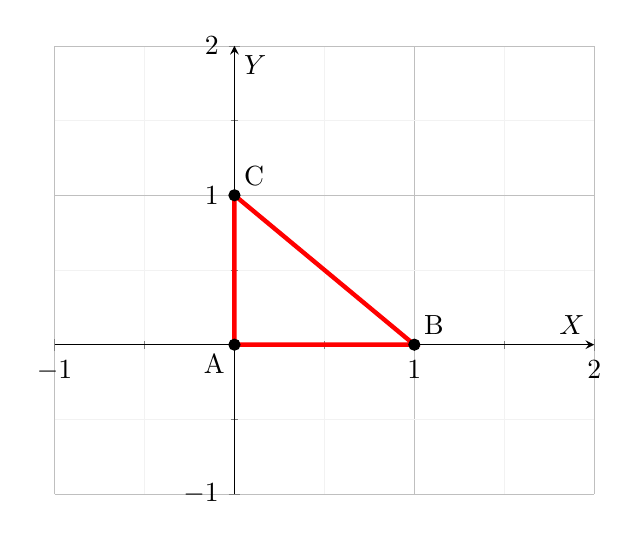
\begin{tikzpicture}
            \begin{axis}[
                axis lines=center,
                xlabel=$X$, ylabel=$Y$,
                xmin=-1, xmax=2,
                ymin=-1, ymax=2,
                xtick={-1,...,2},
                ytick={-1,...,2},
                grid=both,
                grid style={line width=.1pt, draw=gray!10},
                major grid style={line width=.2pt,draw=gray!50},
                minor tick num=1,
                clip=false
            ]
                \addplot[red, ultra thick] coordinates {(0,0) (1,0) (0,1) (0,0)};
                \node[below left] at (axis cs:0,0) {A};
                \node[above right] at (axis cs:1,0) {B};
                \node[above right] at (axis cs:0,1) {C};
                \addplot[only marks,black] coordinates {(0,0) (1,0) (0,1)};
            \end{axis}
        \end{tikzpicture}
    \end{figure}

    Tenemos que dos de sus medianas son:
    \begin{align*}
        M_a & \equiv y=x \equiv (0,0) + \cc{L}\left\{(1,1)\right\}\\
        M_b & \equiv y=-\frac{x}{2}+1 \equiv (1,0) + \cc{L}\left\{(2,-1)\right\}
    \end{align*}

    Por tanto, el baricentro es el punto de intersección de ambas rectas:
    \begin{equation*}
        B=M_a \cap M_b = \left(\frac{1}{3}, \frac{1}{3} \right)
    \end{equation*}

    Tenemos que dos de sus alturas son:
    \begin{align*}
        H_c & \equiv x=0 \equiv (0,0) + \cc{L}\left\{(0, 1)\right\}\\
        H_b & \equiv y=0 \equiv (0,0) + \cc{L}\left\{(1,0)\right\}
    \end{align*}

    Por tanto, el ortocentro es el punto de intersección de ambas rectas:
    \begin{equation*}
        O=H_c \cap H_b = (0,0)
    \end{equation*}

    Tenemos que dos de sus mediatrices son:
    \begin{align*}
        R_c & \equiv x=\frac{1}{2} \equiv \left(\frac{1}{2}, 0\right) + \cc{L}\left\{(0,1)\right\}\\
        R_b & \equiv y=\frac{1}{2} \equiv \left(0, \frac{1}{2}\right) + \cc{L}\left\{(1,0)\right\}
    \end{align*}

    Por tanto, el circuncentro es el punto de intersección de ambas rectas:
    \begin{equation*}
        C=R_c \cap R_b = \left(\frac{1}{2}, \frac{1}{2}\right)
    \end{equation*}

    Para el incentro, no se ve de forma directa. Una de sus bisectrices es la recta $B_a \equiv y=x \equiv (0,0) + \cc{L}\left\{(1,1)\right\}$
    Calculamos ahora $B_c$. Tenemos que $\vec{ca} = (0,-1)$ y $\vec{cb} = \frac{1}{\sqrt{2}}(1,-1)$. Por tanto:
    \begin{equation*}
        v_c = \frac{\vec{ca}}{\left\|\vec{ca}\right\|} + \frac{\vec{cb}}{\left\|\vec{cb}\right\|} = (0,-1) + \frac{1}{\sqrt{2}}(1,-1) = \left(\frac{1}{\sqrt{2}}, -1-\frac{1}{\sqrt{2}}\right)
    \end{equation*}

    Por tanto, la bisectriz $B_c$ es:
    \begin{equation*}
        B_c = (0,1) + \cc{L}\left\{\left(\frac{1}{\sqrt{2}}, -1-\frac{1}{\sqrt{2}}\right)\right\}
    \end{equation*}

    Tenemos que:
    \begin{equation*}
        I=B_a\cap B_c = \left\{\left(\frac{\lm}{\sqrt{2}}, 1-\lm -\frac{\lm}{\sqrt{2}}\right)\in \bb{R}^2 \mid \frac{\lm}{\sqrt{2}} = 1 -\lm -\frac{\lm}{\sqrt{2}}\right\}
        = \left(\frac{\sqrt{2}-1}{\sqrt{2}},\frac{\sqrt{2}-1}{\sqrt{2}}\right)
    \end{equation*}
\end{ejercicio}

\begin{ejercicio}
    ¿Está el incentro de cualquier triángulo alineado con el baricentro, ortocentro y circuncentro?\\

    No, no tiene por qué. Como contraejemplo, veamos el triángulo de vértices $(0,0)$, $(2,0)$ y $(0,1)$.
    \begin{figure}[H]
        \centering
        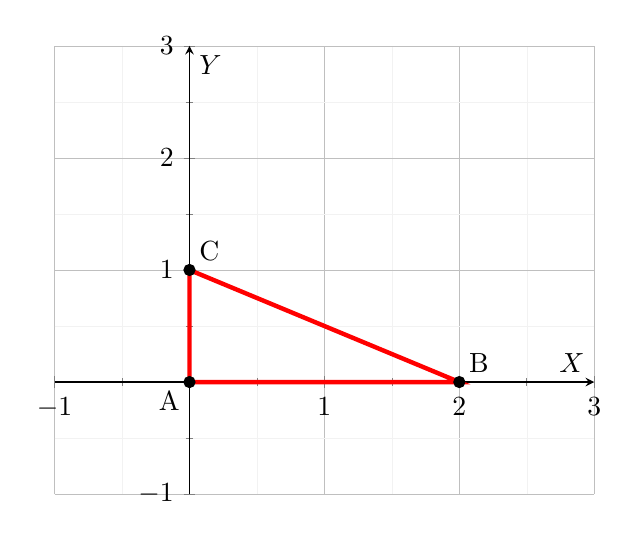
\begin{tikzpicture}
            \begin{axis}[
                axis lines=center,
                xlabel=$X$, ylabel=$Y$,
                xmin=-1, xmax=3,
                ymin=-1, ymax=3,
                xtick={-1,...,3},
                ytick={-1,...,3},
                grid=both,
                grid style={line width=.1pt, draw=gray!10},
                major grid style={line width=.2pt,draw=gray!50},
                minor tick num=1,
                clip=false
            ]
                \addplot[red, ultra thick] coordinates {(0,0) (2,0) (0,1) (0,0)};
                \node[below left] at (axis cs:0,0) {A};
                \node[above right] at (axis cs:2,0) {B};
                \node[above right] at (axis cs:0,1) {C};
                \addplot[only marks,black] coordinates {(0,0) (2,0) (0,1)};
            \end{axis}
        \end{tikzpicture}
    \end{figure}
    Se ve de forma directa que el circuncentro es el punto $C=\left(1,\frac{1}{2}\right)$, y el ortocentro es el origen $O=(0,0)$. Calculemos el incentro.
    
    Una de sus bisectrices es la recta $B_a \equiv y=x \equiv (0,0) + \cc{L}\left\{(1,1)\right\}$
    Calculamos ahora $B_c$. Tenemos que $\vec{ca} = (0,-1)$ y $\vec{cb} = \frac{1}{\sqrt{5}}(2,-1)$. Por tanto:
    \begin{equation*}
        v_c = \frac{\vec{ca}}{\left\|\vec{ca}\right\|} + \frac{\vec{cb}}{\left\|\vec{cb}\right\|} = (0,-1) + \frac{1}{\sqrt{5}}(2,-1) = \left(\frac{2}{\sqrt{5}}, -1-\frac{1}{\sqrt{5}}\right)
    \end{equation*}

    Por tanto, la bisectriz $B_c$ es:
    \begin{equation*}
        B_c = (0,1) + \cc{L}\left\{\left(\frac{2}{\sqrt{5}}, -1-\frac{1}{\sqrt{5}}\right)\right\}
    \end{equation*}

    Tenemos que:
    \begin{equation*}
        I=B_a\cap B_c = \left\{\left(\frac{2\lm}{\sqrt{5}}, 1-\lm -\frac{\lm}{\sqrt{5}}\right)\in \bb{R}^2 \mid \frac{2\lm}{\sqrt{5}} = 1 -\lm -\frac{\lm}{\sqrt{5}}\right\}
        = \left(\frac{3-\sqrt{5}}{2},\frac{3-\sqrt{5}}{2}\right)
    \end{equation*}

    Supongamos ahora que el incentro está alineado con el circuncentro y con el ortocentro. Entonces, $\exists \lm \in \bb{R}$ tal que:
    \begin{equation*}
        \vec{OI} = \lm \vec{OC} \Longrightarrow
        \left(\frac{3-\sqrt{5}}{2},\frac{3-\sqrt{5}}{2}\right) = \lm \left(1,\frac{1}{2}\right)
    \end{equation*}

    Al igualar la primera coordenada, tenemos que $\lm = \dfrac{3-\sqrt{5}}{2}$.
    Sin embargo, al igualar la segunda coordenada, tenemos que $\lm = {3-\sqrt{5}}$, lo cual es un absurdo, por lo que no pueden estar alineados.\\

    Por tanto, aunque el baricentro, el ortocentro y el circuncentro de un triángulo siempre están alineados en la Recta de Euler, el incentro no tiene por qué estarlo.
    En el siguiente ejercicio veremos que, en un triángulo isósceles, los 4 puntos notables de un triángulo están alineados.
\end{ejercicio}

\begin{ejercicio}[Ejercicio de Examen 2022-23]
    Demostrar que, en un triángulo isósceles, los 4 puntos notables de un triángulo están alineados.

    \begin{figure}[H]
        \centering
        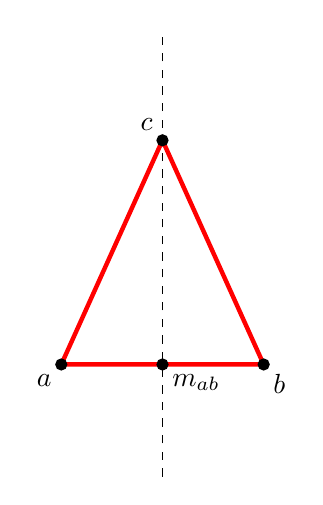
\begin{tikzpicture}
            \begin{axis}[
                axis lines=none,
                xlabel=$X$, ylabel=$Y$,
                xmin=-1, xmax=3,
                ymin=-1, ymax=3,
                grid=both,
                grid style={line width=.1pt, draw=gray!10},
                major grid style={line width=.2pt,draw=gray!50},
                minor tick num=1,
                clip=false
            ]
                \addplot[red, ultra thick] coordinates {(0,0) (0.75,2) (1.5,0) (0,0)};
                \node[below left] at (axis cs:0,0) {$a$};
                \node[below right] at (axis cs:1.5,0) {$b$};
                \node[above left] at (axis cs:0.75,2) {$c$};
                \node[below right] at (axis cs:0.75,0) {$m_{ab}$};
                \addplot[only marks,black] coordinates {(0,0) (0.75,2) (1.5,0) (0.75,0)};

                % Recta x=0.75
                \addplot[dashed] coordinates {(0.75,-1) (0.75,3)};
            \end{axis}
        \end{tikzpicture}
    \end{figure}

    Sea $\bb{E}$ un espacio afín euclídeo, y sea $T=\{a,b,c\}\subset \bb{E}$ un triángulo isósceles con vértices $a,b,c$.
    Supongamos sin pérdida de generalidad que es isósceles por el lado $[a,b]$. Es decir, que $d(a,c) = d(b,c)$.


    Veamos en primer lugar que la mediatriz del lado $[a,b]$ coincide con la bisectriz del ángulo $\widehat{c}$. Es decir, que $R_{c} = B_c$.
    De forma evidente, tenemos que $c\in B_c$. Además, como el triángulo es isósceles, tenemos que $d(a,c) = d(b,c)$, por lo que $c\in R_c$.
    De forma similar, es directo ver que $m_{ab}\in R_c$. Veamos ahora que $m_{ab}\in B_c$:
    \begin{align*}
        \vec{cm_{ab}} &= m_{ab} - c = \cancel{c}+\frac{1}{2}\left(\vec{ca} + \vec{cb}\right) - \cancel{c} = \frac{1}{2}\left(\vec{ca} + \vec{cb}\right)
        = \frac{1}{2} \cdot \frac{\left\|\vec{ca}\right\|}{\left\|\vec{ca}\right\|}\cdot \left(\vec{ca} + \vec{cb}\right)
        =\\&= \frac{1}{2} \cdot \left\|\vec{ca}\right\| \left(\frac{\vec{ca}}{\left\|\vec{ca}\right\|} + \frac{\vec{cb}}{\left\|\vec{ca}\right\|}\right)
        \AstIg \frac{1}{2} \cdot \left\|\vec{ca}\right\| \left(\frac{\vec{ca}}{\left\|\vec{ca}\right\|} + \frac{\vec{cb}}{\left\|\vec{cb}\right\|}\right) \in \vec{B_c}
    \end{align*}
    donde en $(\ast)$ hemos usado que, como el triángulo es isósceles, $d(c,a)=d(b,c)$.

    Por tanto, tenemos que $m_{ab},c \in R_c \cap B_c$, con $m_{ab}\neq c$, por lo que $R_c = B_c$. Veamos ahora que la altura respecto del vértice $c$ coincide con la bisectriz del ángulo $\widehat{c}$,
    es decir, que $H_c = B_c$. De forma evidente, tenemos que $c\in B_c\cap H_c$. Además, ya hemos visto que $m_{ab}\in B_c$. Veamos ahora que $m_{ab}\in H_c$:
    \begin{align*}
        \left\langle \vec{cm_{ab}}, \vec{ab}\right\rangle &=
        \left\langle m_{ab}-c, \vec{ab}\right\rangle = \left\langle \cancel{c}+\frac{1}{2}\left(\vec{ca} + \vec{cb}\right) - \cancel{c}, \vec{ab}\right\rangle
        = \frac{1}{2}\left\langle \vec{ca} + \vec{cb}, \vec{ab}\right\rangle =\\
        &= \frac{1}{2}\left\langle -\vec{ac} + \vec{cb}, \vec{ac} + \vec{cb}\right\rangle =\\
        &= \frac{1}{2}\left[-\left\|\vec{ac}\right\|^2 + \left\|\vec{cb}\right\|^2 - \cancel{\left\langle \vec{ac}, \vec{cb}\right\rangle} + \cancel{\left\langle \vec{cb}, \vec{ac}\right\rangle}\right]
        \AstIg 0
    \end{align*}
    donde, en la última igualdad, hemos usado que, como el triángulo es isósceles, $d(c,a)=d(b,c)$. Por tanto, $\vec{cm_{ab}}\perp \vec{ab}$ y, por tanto, $m_{ab}\in H_c$.

    Por tanto, tenemos que $m_{ab},c \in H_c \cap B_c \cap R_c$, con $m_{ab}\neq C$, por lo que $R_c = B_c = H_c$. Como $C,O,I\in R_c=B_c=H_c$, tenemos que $C,O,I$ están alineados en dicha recta.
    Es decir, como coinciden la altura, la bisectriz y la mediatriz asociadas al vértice $C$, entonces el circuncentro, el ortocentro y el incentro están alineados.

    Como además el baricentro siempre está alineado con el circuncentro y el ortocentro por el Teorema de Euler en la Recta de Euler, tenemos que los 4 puntos notables de un triángulo isósceles están alineados en la Recta de Euler.
\end{ejercicio}



\begin{ejercicio}
    Construye explícitamente, si es posible,
    un movimiento rígido directo $f$ del espacio afín euclídeo que cumpla
    $f(2,0,0)=(1,1,1)$, no tenga puntos fijos, y no sea una traslación.

    Como es un movimiento rígido directo en el espacio y no tiene puntos fijos, ha de
    ser un movimiento helicoidal. Sea el giro respecto de la recta $L$ de ángulo no orientado $\theta \in ]0, \pi]$ y vector de traslación $v\in \vec{L}\setminus \{0\}$.

    Supongamos $\vec{L}=\cc{L}\{(0,0,1)\}$, y $v=(0,0,1)$. Entonces, el giro es $G_{\theta, L}$, y la traslación es $t_v$.
    Necesitamos entonces que $G_{\theta, L}(2,0,0) = (1,1,0)$. Veámoslo gráficamente:
    \begin{figure}[H]
        \centering
        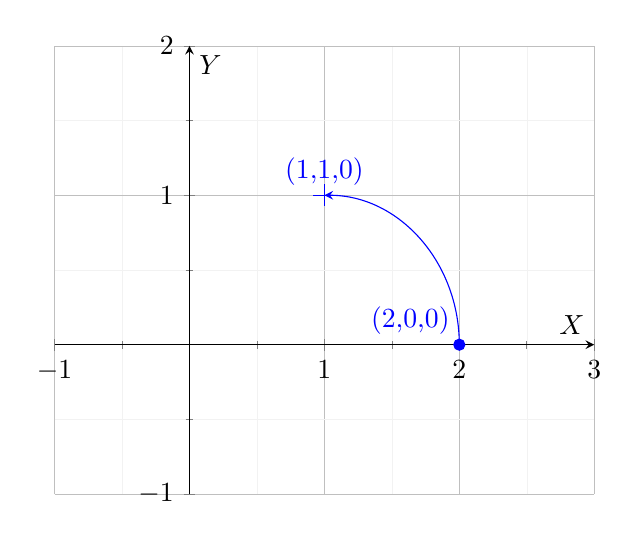
\begin{tikzpicture}
            \shorthandoff{"}
            \begin{axis}[
                axis lines=center,
                xlabel=$X$, ylabel=$Y$,
                xmin=-1, xmax=3,
                ymin=-1, ymax=2,
                xtick={-1,...,3},
                ytick={-1,...,2},
                grid=both,
                grid style={line width=.1pt, draw=gray!10},
                major grid style={line width=.2pt,draw=gray!50},
                minor tick num=1,
                clip=false
            ]
                %\addplot[only marks,red, nodes near coords={(1,0,0)}, every node near coord/.append style={red, anchor=west}] coordinates {(0,1)};
                %\addplot[only marks,red] coordinates {(0,1)};
                
                \addplot[only marks,blue, nodes near coords={(2,0,0)}, every node near coord/.append style={blue, anchor=south east}] coordinates {(2,0)};
                \addplot[only marks,blue] coordinates {(2,0)};

                \addplot[only marks,blue, nodes near coords={(1,1,0)}, every node near coord/.append style={blue, anchor=south}] coordinates {(1,1)};
                \addplot[only marks,blue, mark=+, mark options={scale=2}] coordinates {(1,1)};
                \draw[blue, stealth-] (axis cs:1,1) arc[start angle=90, end angle=0, radius=1];
            \end{axis}
            \shorthandon{"}
        \end{tikzpicture}
        \caption{Plano $L_{(2,0,0)}^\perp$.}
    \end{figure}

    Por tanto, gráficamente vemos que se trata de un giro de ángulo no orientado $\theta = \frac{\pi}{2}$ respecto del eje $L=(1,0,0) + \cc{L}\{(0,0,1)\}$,
    y una traslación según el vector $v=(0,0,1)$.
\end{ejercicio}